\documentclass[a4paper]{book}
\usepackage{makeidx}
\usepackage{natbib}
\usepackage{graphicx}
\usepackage{multicol}
\usepackage{float}
\usepackage{listings}
\usepackage{color}
\usepackage{ifthen}
\usepackage[table]{xcolor}
\usepackage{textcomp}
\usepackage{alltt}
\usepackage{ifpdf}
\ifpdf
\usepackage[pdftex,
            pagebackref=true,
            colorlinks=true,
            linkcolor=blue,
            unicode
           ]{hyperref}
\else
\usepackage[ps2pdf,
            pagebackref=true,
            colorlinks=true,
            linkcolor=blue,
            unicode
           ]{hyperref}
\usepackage{pspicture}
\fi
\usepackage[utf8]{inputenc}
\usepackage{polski}
\usepackage[T1]{fontenc}

\usepackage{mathptmx}
\usepackage[scaled=.90]{helvet}
\usepackage{courier}
\usepackage{sectsty}
\usepackage[titles]{tocloft}
\usepackage{doxygen}
\lstset{language=C++,inputencoding=utf8,basicstyle=\footnotesize,breaklines=true,breakatwhitespace=true,tabsize=8,numbers=left }
\makeindex
\setcounter{tocdepth}{3}
\renewcommand{\footrulewidth}{0.4pt}
\renewcommand{\familydefault}{\sfdefault}
\hfuzz=15pt
\setlength{\emergencystretch}{15pt}
\hbadness=750
\tolerance=750
\begin{document}
\hypersetup{pageanchor=false,citecolor=blue}
\begin{titlepage}
\vspace*{7cm}
\begin{center}
{\Large \-P\-A\-M\-S\-I -\/ pwilkosz \\[1ex]\large 1.\-0 }\\
\vspace*{1cm}
{\large \-Wygenerowano przez Doxygen 1.7.6.1}\\
\vspace*{0.5cm}
{\small Sun Mar 23 2014 14:06:28}\\
\end{center}
\end{titlepage}
\clearemptydoublepage
\pagenumbering{roman}
\tableofcontents
\clearemptydoublepage
\pagenumbering{arabic}
\hypersetup{pageanchor=true,citecolor=blue}
\chapter{\-Indeks klas}
\section{\-Hierarchia klas}
\-Ta lista dziedziczenia posortowana jest z grubsza, choć nie całkowicie, alfabetycznie\-:\begin{DoxyCompactList}
\item \contentsline{section}{algorytm}{\pageref{classalgorytm}}{}
\begin{DoxyCompactList}
\item \contentsline{section}{h\-\_\-sort}{\pageref{classh__sort}}{}
\item \contentsline{section}{kolejka\-\_\-lista}{\pageref{classkolejka__lista}}{}
\item \contentsline{section}{kolejka\-\_\-tablica}{\pageref{classkolejka__tablica}}{}
\item \contentsline{section}{m\-\_\-sort}{\pageref{classm__sort}}{}
\item \contentsline{section}{mnozenie}{\pageref{classmnozenie}}{}
\item \contentsline{section}{q\-\_\-sort}{\pageref{classq__sort}}{}
\item \contentsline{section}{stos\-\_\-lista}{\pageref{classstos__lista}}{}
\item \contentsline{section}{stos\-\_\-tablica}{\pageref{classstos__tablica}}{}
\end{DoxyCompactList}
\item \contentsline{section}{operacje}{\pageref{classoperacje}}{}
\item \contentsline{section}{queue\-\_\-array$<$ \-T\-Y\-P $>$}{\pageref{classqueue__array}}{}
\item \contentsline{section}{queue\-\_\-list$<$ \-T\-Y\-P $>$}{\pageref{classqueue__list}}{}
\item \contentsline{section}{stack\-\_\-array$<$ \-T\-Y\-P $>$}{\pageref{classstack__array}}{}
\item \contentsline{section}{stack\-\_\-list$<$ \-T\-Y\-P $>$}{\pageref{classstack__list}}{}
\end{DoxyCompactList}

\chapter{\-Indeks klas}
\section{\-Lista klas}
\-Tutaj znajdują się klasy, struktury, unie i interfejsy wraz z ich krótkimi opisami\-:\begin{DoxyCompactList}
\item\contentsline{section}{\hyperlink{classalgorytm}{algorytm} \\*\-Definicja klasy algorytm \-Jest to klasa bazowa, ktora ma za zadanie wczytac, przetworzyc i porownac dane z plikiem wzorcowym }{\pageref{classalgorytm}}{}
\item\contentsline{section}{\hyperlink{classmnozenie}{mnozenie} \\*\-Modeluje algorytm dokonujacy mnozenia kazdego elementu pliku wejsciowego przez 2 }{\pageref{classmnozenie}}{}
\item\contentsline{section}{\hyperlink{classoperacje}{operacje} \\*\-Klasa modeluje tablice z danymi i metody sluzace do operacji na niej }{\pageref{classoperacje}}{}
\end{DoxyCompactList}

\chapter{\-Indeks plików}
\section{Lista plików}
Tutaj znajduje się lista wszystkich plików z ich krótkimi opisami\-:\begin{DoxyCompactList}
\item\contentsline{section}{\hyperlink{algorytm_8cpp}{algorytm.\-cpp} \\*Plik zawiera definicje metod klas zdefiniowanych w pliku \hyperlink{algorytm_8hh}{algorytm.\-hh} }{\pageref{algorytm_8cpp}}{}
\item\contentsline{section}{\hyperlink{algorytm_8hh}{algorytm.\-hh} \\*Definicja klas wykonujacych operacje na zestawie danych wejsciowych }{\pageref{algorytm_8hh}}{}
\item\contentsline{section}{\hyperlink{drzewo_8hh}{drzewo.\-hh} }{\pageref{drzewo_8hh}}{}
\item\contentsline{section}{\hyperlink{graf_8cpp}{graf.\-cpp} }{\pageref{graf_8cpp}}{}
\item\contentsline{section}{\hyperlink{graf_8hh}{graf.\-hh} }{\pageref{graf_8hh}}{}
\item\contentsline{section}{\hyperlink{hashtab_8hh}{hashtab.\-hh} }{\pageref{hashtab_8hh}}{}
\item\contentsline{section}{\hyperlink{kolejka_8hh}{kolejka.\-hh} \\*Plik zawiera definicje klasy Kolejka Zaimplementowanej na 2 sposoby }{\pageref{kolejka_8hh}}{}
\item\contentsline{section}{\hyperlink{main_8cpp}{main.\-cpp} \\*Plik glowny }{\pageref{main_8cpp}}{}
\item\contentsline{section}{\hyperlink{operacje_8cpp}{operacje.\-cpp} }{\pageref{operacje_8cpp}}{}
\item\contentsline{section}{\hyperlink{operacje_8hh}{operacje.\-hh} }{\pageref{operacje_8hh}}{}
\item\contentsline{section}{\hyperlink{simplex_8cpp}{simplex.\-cpp} }{\pageref{simplex_8cpp}}{}
\item\contentsline{section}{\hyperlink{simplex_8hh}{simplex.\-hh} }{\pageref{simplex_8hh}}{}
\item\contentsline{section}{\hyperlink{statystyki_8cpp}{statystyki.\-cpp} }{\pageref{statystyki_8cpp}}{}
\item\contentsline{section}{\hyperlink{statystyki_8hh}{statystyki.\-hh} \\*Plik zawiera dekalracje funkcji odpowiedzialnych za przeprowadznaie statystyk }{\pageref{statystyki_8hh}}{}
\item\contentsline{section}{\hyperlink{stos_8hh}{stos.\-hh} \\*Plik zawiera definicje klasy {\ttfamily Stos} Zaimplementowana na 2 sposoby }{\pageref{stos_8hh}}{}
\item\contentsline{section}{\hyperlink{str__operacje_8cpp}{str\-\_\-operacje.\-cpp} }{\pageref{str__operacje_8cpp}}{}
\item\contentsline{section}{\hyperlink{str__operacje_8hh}{str\-\_\-operacje.\-hh} }{\pageref{str__operacje_8hh}}{}
\item\contentsline{section}{\hyperlink{tablica__asocjacyjna_8hh}{tablica\-\_\-asocjacyjna.\-hh} }{\pageref{tablica__asocjacyjna_8hh}}{}
\end{DoxyCompactList}

\chapter{\-Dokumentacja klas}
\hypertarget{classalgorytm}{\section{\-Dokumentacja klasy algorytm}
\label{classalgorytm}\index{algorytm@{algorytm}}
}


\-Definicja klasy algorytm \-Jest to klasa bazowa, ktora ma za zadanie wczytac, przetworzyc i porownac plik z plikiem wzorcowym.  




{\ttfamily \#include $<$algorytm.\-hh$>$}



\-Diagram dziedziczenia dla algorytm
\nopagebreak
\begin{figure}[H]
\begin{center}
\leavevmode
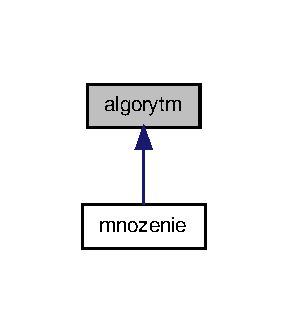
\includegraphics[width=138pt]{classalgorytm__inherit__graph}
\end{center}
\end{figure}
\subsection*{\-Metody publiczne}
\begin{DoxyCompactItemize}
\item 
\hyperlink{classalgorytm_a138ed27849535b192fec3d2e9f6a644f}{algorytm} (const char $\ast$plik1, const char $\ast$plik2)
\begin{DoxyCompactList}\small\item\em konstruktor kopiujacy -\/ przekazuje informacje o nazwach plikow, ktore zapisywane sa do pol klasy \end{DoxyCompactList}\item 
virtual void \hyperlink{classalgorytm_a85ba543fad39e8987bbda4ee698b5fec}{wykonaj} ()
\begin{DoxyCompactList}\small\item\em funkcja dokonuje operacji na pliku wejsciowym \end{DoxyCompactList}\item 
bool \hyperlink{classalgorytm_a167adca6239e12cb5d362fd7c905dde0}{porownaj} ()
\begin{DoxyCompactList}\small\item\em porownuje przetworzony plik z plikiem wzorcowym \end{DoxyCompactList}\item 
int \hyperlink{classalgorytm_acbd9260a0b2055acee485f737b960992}{ile\-\_\-danych} ()
\item 
vector$<$ float $>$ \hyperlink{classalgorytm_a244d9cbf20639faf0b60ae6cdae3c657}{jaki\-\_\-czas} ()
\end{DoxyCompactItemize}
\subsection*{\-Atrybuty publiczne}
\begin{DoxyCompactItemize}
\item 
vector$<$ float $>$ \hyperlink{classalgorytm_aac9e2179e0e956dbe0dc1239ebadb2e4}{czas}
\begin{DoxyCompactList}\small\item\em zawiera wyniki dzialania algorytmu \end{DoxyCompactList}\end{DoxyCompactItemize}
\subsection*{\-Atrybuty chronione}
\begin{DoxyCompactItemize}
\item 
int \hyperlink{classalgorytm_a2778c37f0ec06a30b7d494501c40e91a}{n}
\begin{DoxyCompactList}\small\item\em zawiera informacje o ilosci liczb w pliku \end{DoxyCompactList}\item 
const char $\ast$ \hyperlink{classalgorytm_ab911ca0437df967d0240651855e5a2a3}{plik\-We}
\begin{DoxyCompactList}\small\item\em zawiera nazwe pliku wejsciowego \end{DoxyCompactList}\item 
const char $\ast$ \hyperlink{classalgorytm_a19c2be15efb3e5e34bf177d50b746d93}{plik\-Wz}
\begin{DoxyCompactList}\small\item\em zawiera nazwe pliku wzorcowego \end{DoxyCompactList}\end{DoxyCompactItemize}


\subsection{\-Opis szczegółowy}
\-Definicja klasy algorytm \-Jest to klasa bazowa, ktora ma za zadanie wczytac, przetworzyc i porownac plik z plikiem wzorcowym. 

\-Definicja w linii 32 pliku algorytm.\-hh.



\subsection{\-Dokumentacja konstruktora i destruktora}
\hypertarget{classalgorytm_a138ed27849535b192fec3d2e9f6a644f}{\index{algorytm@{algorytm}!algorytm@{algorytm}}
\index{algorytm@{algorytm}!algorytm@{algorytm}}
\subsubsection[{algorytm}]{\setlength{\rightskip}{0pt plus 5cm}{\bf algorytm\-::algorytm} (
\begin{DoxyParamCaption}
\item[{const char $\ast$}]{plik1, }
\item[{const char $\ast$}]{plik2}
\end{DoxyParamCaption}
)\hspace{0.3cm}{\ttfamily  \mbox{[}inline\mbox{]}}}}\label{classalgorytm_a138ed27849535b192fec3d2e9f6a644f}


konstruktor kopiujacy -\/ przekazuje informacje o nazwach plikow, ktore zapisywane sa do pol klasy 


\begin{DoxyParams}{\-Parametry}
{\em plik1} & -\/ plik wejsciowy \\
\hline
{\em plik2} & -\/ plik wzorcowy \\
\hline
\end{DoxyParams}


\-Definicja w linii 56 pliku algorytm.\-hh.



\subsection{\-Dokumentacja funkcji składowych}
\hypertarget{classalgorytm_acbd9260a0b2055acee485f737b960992}{\index{algorytm@{algorytm}!ile\-\_\-danych@{ile\-\_\-danych}}
\index{ile\-\_\-danych@{ile\-\_\-danych}!algorytm@{algorytm}}
\subsubsection[{ile\-\_\-danych}]{\setlength{\rightskip}{0pt plus 5cm}int {\bf algorytm\-::ile\-\_\-danych} (
\begin{DoxyParamCaption}
{}
\end{DoxyParamCaption}
)}}\label{classalgorytm_acbd9260a0b2055acee485f737b960992}
\begin{DoxyReturn}{\-Zwraca}
ilosc liczb wejsciowych 
\end{DoxyReturn}


\-Definicja w linii 16 pliku algorytm.\-cpp.

\hypertarget{classalgorytm_a244d9cbf20639faf0b60ae6cdae3c657}{\index{algorytm@{algorytm}!jaki\-\_\-czas@{jaki\-\_\-czas}}
\index{jaki\-\_\-czas@{jaki\-\_\-czas}!algorytm@{algorytm}}
\subsubsection[{jaki\-\_\-czas}]{\setlength{\rightskip}{0pt plus 5cm}vector$<$ float $>$ {\bf algorytm\-::jaki\-\_\-czas} (
\begin{DoxyParamCaption}
{}
\end{DoxyParamCaption}
)}}\label{classalgorytm_a244d9cbf20639faf0b60ae6cdae3c657}


\-Definicja w linii 19 pliku algorytm.\-cpp.

\hypertarget{classalgorytm_a167adca6239e12cb5d362fd7c905dde0}{\index{algorytm@{algorytm}!porownaj@{porownaj}}
\index{porownaj@{porownaj}!algorytm@{algorytm}}
\subsubsection[{porownaj}]{\setlength{\rightskip}{0pt plus 5cm}bool {\bf algorytm\-::porownaj} (
\begin{DoxyParamCaption}
{}
\end{DoxyParamCaption}
)}}\label{classalgorytm_a167adca6239e12cb5d362fd7c905dde0}


porownuje przetworzony plik z plikiem wzorcowym 

\begin{DoxyReturn}{\-Zwraca}
true -\/ gdy pliki zgodne false -\/ w przeciwnym przypadku 
\end{DoxyReturn}


\-Definicja w linii 23 pliku algorytm.\-cpp.



\-Oto graf wywoływań tej funkcji\-:
\nopagebreak
\begin{figure}[H]
\begin{center}
\leavevmode
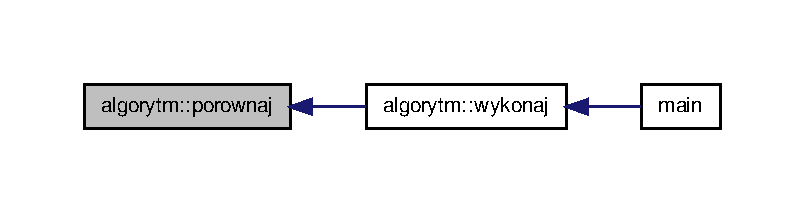
\includegraphics[width=350pt]{classalgorytm_a167adca6239e12cb5d362fd7c905dde0_icgraph}
\end{center}
\end{figure}


\hypertarget{classalgorytm_a85ba543fad39e8987bbda4ee698b5fec}{\index{algorytm@{algorytm}!wykonaj@{wykonaj}}
\index{wykonaj@{wykonaj}!algorytm@{algorytm}}
\subsubsection[{wykonaj}]{\setlength{\rightskip}{0pt plus 5cm}void {\bf algorytm\-::wykonaj} (
\begin{DoxyParamCaption}
{}
\end{DoxyParamCaption}
)\hspace{0.3cm}{\ttfamily  \mbox{[}virtual\mbox{]}}}}\label{classalgorytm_a85ba543fad39e8987bbda4ee698b5fec}


funkcja dokonuje operacji na pliku wejsciowym 



\-Reimplementowana w \hyperlink{classmnozenie_a2c5dc64610bb16af0ef18d142d6af2c0}{mnozenie}.



\-Definicja w linii 7 pliku algorytm.\-cpp.



\subsection{\-Dokumentacja atrybutów składowych}
\hypertarget{classalgorytm_aac9e2179e0e956dbe0dc1239ebadb2e4}{\index{algorytm@{algorytm}!czas@{czas}}
\index{czas@{czas}!algorytm@{algorytm}}
\subsubsection[{czas}]{\setlength{\rightskip}{0pt plus 5cm}vector$<$float$>$ {\bf algorytm\-::czas}}}\label{classalgorytm_aac9e2179e0e956dbe0dc1239ebadb2e4}


zawiera wyniki dzialania algorytmu 



\-Definicja w linii 50 pliku algorytm.\-hh.

\hypertarget{classalgorytm_a2778c37f0ec06a30b7d494501c40e91a}{\index{algorytm@{algorytm}!n@{n}}
\index{n@{n}!algorytm@{algorytm}}
\subsubsection[{n}]{\setlength{\rightskip}{0pt plus 5cm}int {\bf algorytm\-::n}\hspace{0.3cm}{\ttfamily  \mbox{[}protected\mbox{]}}}}\label{classalgorytm_a2778c37f0ec06a30b7d494501c40e91a}


zawiera informacje o ilosci liczb w pliku 



\-Definicja w linii 37 pliku algorytm.\-hh.

\hypertarget{classalgorytm_ab911ca0437df967d0240651855e5a2a3}{\index{algorytm@{algorytm}!plik\-We@{plik\-We}}
\index{plik\-We@{plik\-We}!algorytm@{algorytm}}
\subsubsection[{plik\-We}]{\setlength{\rightskip}{0pt plus 5cm}const char$\ast$ {\bf algorytm\-::plik\-We}\hspace{0.3cm}{\ttfamily  \mbox{[}protected\mbox{]}}}}\label{classalgorytm_ab911ca0437df967d0240651855e5a2a3}


zawiera nazwe pliku wejsciowego 



\-Definicja w linii 41 pliku algorytm.\-hh.

\hypertarget{classalgorytm_a19c2be15efb3e5e34bf177d50b746d93}{\index{algorytm@{algorytm}!plik\-Wz@{plik\-Wz}}
\index{plik\-Wz@{plik\-Wz}!algorytm@{algorytm}}
\subsubsection[{plik\-Wz}]{\setlength{\rightskip}{0pt plus 5cm}const char$\ast$ {\bf algorytm\-::plik\-Wz}\hspace{0.3cm}{\ttfamily  \mbox{[}protected\mbox{]}}}}\label{classalgorytm_a19c2be15efb3e5e34bf177d50b746d93}


zawiera nazwe pliku wzorcowego 



\-Definicja w linii 45 pliku algorytm.\-hh.



\-Dokumentacja dla tej klasy została wygenerowana z plików\-:\begin{DoxyCompactItemize}
\item 
\hyperlink{algorytm_8hh}{algorytm.\-hh}\item 
\hyperlink{algorytm_8cpp}{algorytm.\-cpp}\end{DoxyCompactItemize}

\hypertarget{classh__sort}{\section{\-Dokumentacja klasy h\-\_\-sort}
\label{classh__sort}\index{h\-\_\-sort@{h\-\_\-sort}}
}


klasa reprezentuje dane poddane sortowaniu przez kopcowanie  




{\ttfamily \#include $<$algorytm.\-hh$>$}



\-Diagram dziedziczenia dla h\-\_\-sort\nopagebreak
\begin{figure}[H]
\begin{center}
\leavevmode
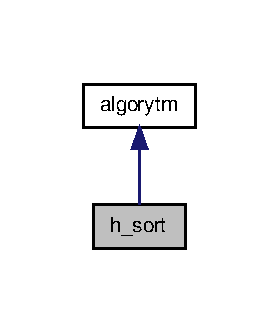
\includegraphics[width=134pt]{classh__sort__inherit__graph}
\end{center}
\end{figure}


\-Diagram współpracy dla h\-\_\-sort\-:\nopagebreak
\begin{figure}[H]
\begin{center}
\leavevmode
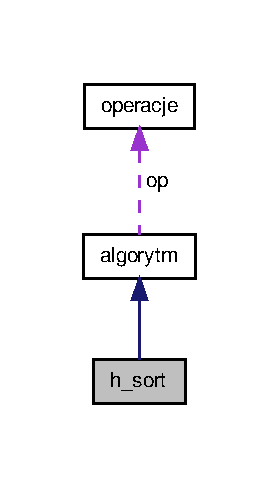
\includegraphics[width=134pt]{classh__sort__coll__graph}
\end{center}
\end{figure}
\subsection*{\-Metody publiczne}
\begin{DoxyCompactItemize}
\item 
\hyperlink{classh__sort_a27a9e6a24497264c3b9e0101f417e4ad}{h\-\_\-sort} (ifstream \&plik1, ifstream \&plik2, int \-N, int \-M)
\begin{DoxyCompactList}\small\item\em konstruktor klasy \end{DoxyCompactList}\item 
float \hyperlink{classh__sort_a496c249e58b48ca10e06266d1f673bd7}{przelicz} ()
\begin{DoxyCompactList}\small\item\em metoda dokonujaca sortowania danych \end{DoxyCompactList}\end{DoxyCompactItemize}


\subsection{\-Opis szczegółowy}
klasa reprezentuje dane poddane sortowaniu przez kopcowanie 

\-Definicja w linii 207 pliku algorytm.\-hh.



\subsection{\-Dokumentacja konstruktora i destruktora}
\hypertarget{classh__sort_a27a9e6a24497264c3b9e0101f417e4ad}{\index{h\-\_\-sort@{h\-\_\-sort}!h\-\_\-sort@{h\-\_\-sort}}
\index{h\-\_\-sort@{h\-\_\-sort}!h_sort@{h\-\_\-sort}}
\subsubsection[{h\-\_\-sort}]{\setlength{\rightskip}{0pt plus 5cm}{\bf h\-\_\-sort\-::h\-\_\-sort} (
\begin{DoxyParamCaption}
\item[{ifstream \&}]{plik1, }
\item[{ifstream \&}]{plik2, }
\item[{int}]{\-N, }
\item[{int}]{\-M}
\end{DoxyParamCaption}
)\hspace{0.3cm}{\ttfamily  \mbox{[}inline\mbox{]}}}}\label{classh__sort_a27a9e6a24497264c3b9e0101f417e4ad}


konstruktor klasy 



\-Definicja w linii 210 pliku algorytm.\-hh.



\subsection{\-Dokumentacja funkcji składowych}
\hypertarget{classh__sort_a496c249e58b48ca10e06266d1f673bd7}{\index{h\-\_\-sort@{h\-\_\-sort}!przelicz@{przelicz}}
\index{przelicz@{przelicz}!h_sort@{h\-\_\-sort}}
\subsubsection[{przelicz}]{\setlength{\rightskip}{0pt plus 5cm}float {\bf h\-\_\-sort\-::przelicz} (
\begin{DoxyParamCaption}
{}
\end{DoxyParamCaption}
)\hspace{0.3cm}{\ttfamily  \mbox{[}virtual\mbox{]}}}}\label{classh__sort_a496c249e58b48ca10e06266d1f673bd7}


metoda dokonujaca sortowania danych 



\-Reimplementowana z \hyperlink{classalgorytm_af3f92bf537b1f2e1f93173983e838449}{algorytm}.



\-Definicja w linii 180 pliku algorytm.\-cpp.



\-Oto graf wywołań dla tej funkcji\-:\nopagebreak
\begin{figure}[H]
\begin{center}
\leavevmode
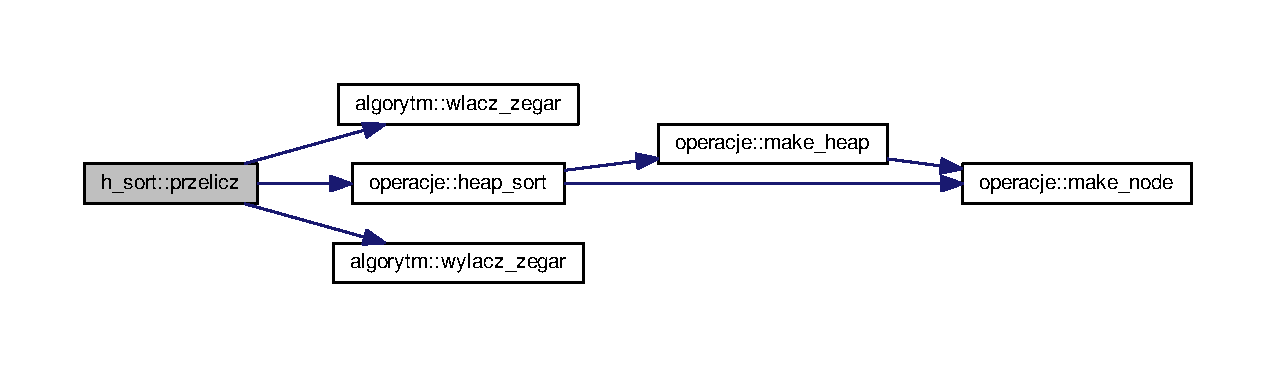
\includegraphics[width=350pt]{classh__sort_a496c249e58b48ca10e06266d1f673bd7_cgraph}
\end{center}
\end{figure}




\-Dokumentacja dla tej klasy została wygenerowana z plików\-:\begin{DoxyCompactItemize}
\item 
\hyperlink{algorytm_8hh}{algorytm.\-hh}\item 
\hyperlink{algorytm_8cpp}{algorytm.\-cpp}\end{DoxyCompactItemize}

\hypertarget{classkolejka__lista}{\section{\-Dokumentacja klasy kolejka\-\_\-lista}
\label{classkolejka__lista}\index{kolejka\-\_\-lista@{kolejka\-\_\-lista}}
}


klasa utworzona na potrzeby pomiaru czasu wypełnienia struktury  




{\ttfamily \#include $<$algorytm.\-hh$>$}



\-Diagram dziedziczenia dla kolejka\-\_\-lista\nopagebreak
\begin{figure}[H]
\begin{center}
\leavevmode
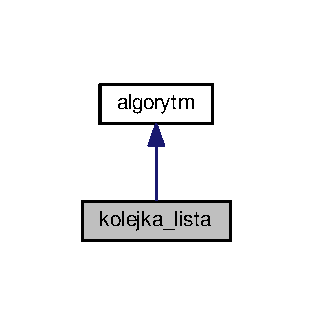
\includegraphics[width=150pt]{classkolejka__lista__inherit__graph}
\end{center}
\end{figure}


\-Diagram współpracy dla kolejka\-\_\-lista\-:\nopagebreak
\begin{figure}[H]
\begin{center}
\leavevmode
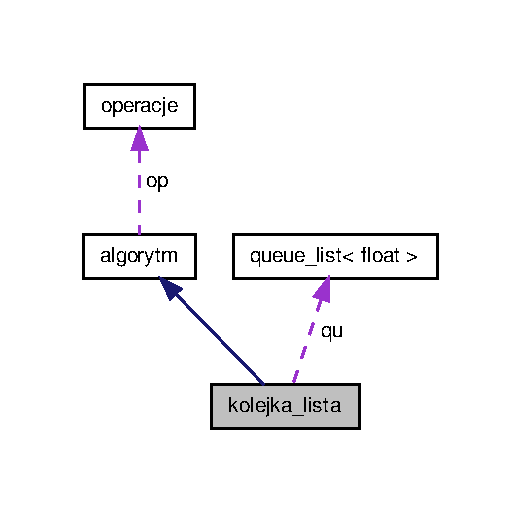
\includegraphics[width=250pt]{classkolejka__lista__coll__graph}
\end{center}
\end{figure}
\subsection*{\-Metody publiczne}
\begin{DoxyCompactItemize}
\item 
\hyperlink{classkolejka__lista_a5472805c319e05803d4841aecfd0c910}{kolejka\-\_\-lista} (ifstream \&plik1, ifstream \&plik2, int \-N, int \-M)
\item 
float \hyperlink{classkolejka__lista_a239ae8bcd2dcee9b79945010e0e32037}{przelicz} ()
\begin{DoxyCompactList}\small\item\em \-Metoda odpowiada za przetworzenie danych wejsciowych zgodnie z zadanym algorytmem. \end{DoxyCompactList}\end{DoxyCompactItemize}
\subsection*{\-Atrybuty prywatne}
\begin{DoxyCompactItemize}
\item 
\hyperlink{classqueue__list}{queue\-\_\-list}$<$ float $>$ \hyperlink{classkolejka__lista_a5e378458ccfc86d903b1a71a8ff5bad8}{qu}
\end{DoxyCompactItemize}


\subsection{\-Opis szczegółowy}
klasa utworzona na potrzeby pomiaru czasu wypełnienia struktury 

\-Definicja w linii 186 pliku algorytm.\-hh.



\subsection{\-Dokumentacja konstruktora i destruktora}
\hypertarget{classkolejka__lista_a5472805c319e05803d4841aecfd0c910}{\index{kolejka\-\_\-lista@{kolejka\-\_\-lista}!kolejka\-\_\-lista@{kolejka\-\_\-lista}}
\index{kolejka\-\_\-lista@{kolejka\-\_\-lista}!kolejka_lista@{kolejka\-\_\-lista}}
\subsubsection[{kolejka\-\_\-lista}]{\setlength{\rightskip}{0pt plus 5cm}{\bf kolejka\-\_\-lista\-::kolejka\-\_\-lista} (
\begin{DoxyParamCaption}
\item[{ifstream \&}]{plik1, }
\item[{ifstream \&}]{plik2, }
\item[{int}]{\-N, }
\item[{int}]{\-M}
\end{DoxyParamCaption}
)\hspace{0.3cm}{\ttfamily  \mbox{[}inline\mbox{]}}}}\label{classkolejka__lista_a5472805c319e05803d4841aecfd0c910}


\-Definicja w linii 189 pliku algorytm.\-hh.



\subsection{\-Dokumentacja funkcji składowych}
\hypertarget{classkolejka__lista_a239ae8bcd2dcee9b79945010e0e32037}{\index{kolejka\-\_\-lista@{kolejka\-\_\-lista}!przelicz@{przelicz}}
\index{przelicz@{przelicz}!kolejka_lista@{kolejka\-\_\-lista}}
\subsubsection[{przelicz}]{\setlength{\rightskip}{0pt plus 5cm}float {\bf kolejka\-\_\-lista\-::przelicz} (
\begin{DoxyParamCaption}
{}
\end{DoxyParamCaption}
)\hspace{0.3cm}{\ttfamily  \mbox{[}virtual\mbox{]}}}}\label{classkolejka__lista_a239ae8bcd2dcee9b79945010e0e32037}


\-Metoda odpowiada za przetworzenie danych wejsciowych zgodnie z zadanym algorytmem. 



\-Reimplementowana z \hyperlink{classalgorytm_af3f92bf537b1f2e1f93173983e838449}{algorytm}.



\-Definicja w linii 143 pliku algorytm.\-cpp.



\-Oto graf wywołań dla tej funkcji\-:\nopagebreak
\begin{figure}[H]
\begin{center}
\leavevmode
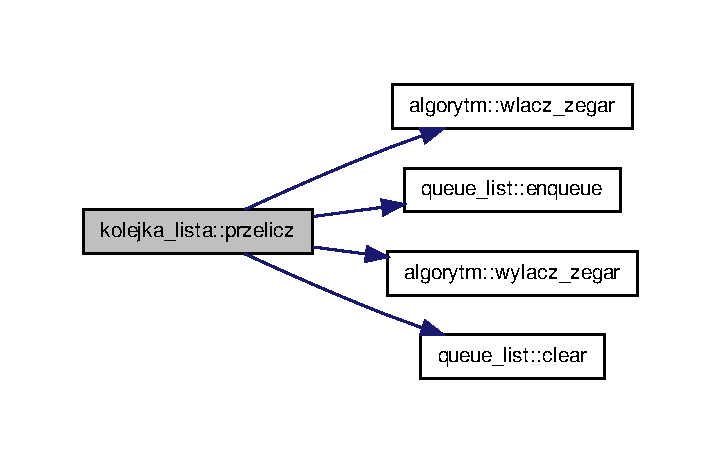
\includegraphics[width=346pt]{classkolejka__lista_a239ae8bcd2dcee9b79945010e0e32037_cgraph}
\end{center}
\end{figure}




\subsection{\-Dokumentacja atrybutów składowych}
\hypertarget{classkolejka__lista_a5e378458ccfc86d903b1a71a8ff5bad8}{\index{kolejka\-\_\-lista@{kolejka\-\_\-lista}!qu@{qu}}
\index{qu@{qu}!kolejka_lista@{kolejka\-\_\-lista}}
\subsubsection[{qu}]{\setlength{\rightskip}{0pt plus 5cm}{\bf queue\-\_\-list}$<$float$>$ {\bf kolejka\-\_\-lista\-::qu}\hspace{0.3cm}{\ttfamily  \mbox{[}private\mbox{]}}}}\label{classkolejka__lista_a5e378458ccfc86d903b1a71a8ff5bad8}


\-Definicja w linii 187 pliku algorytm.\-hh.



\-Dokumentacja dla tej klasy została wygenerowana z plików\-:\begin{DoxyCompactItemize}
\item 
\hyperlink{algorytm_8hh}{algorytm.\-hh}\item 
\hyperlink{algorytm_8cpp}{algorytm.\-cpp}\end{DoxyCompactItemize}

\hypertarget{classkolejka__tablica}{\section{Dokumentacja klasy kolejka\-\_\-tablica}
\label{classkolejka__tablica}\index{kolejka\-\_\-tablica@{kolejka\-\_\-tablica}}
}


klasa utworzona na potrzeby pomiaru czasu wypełnienia struktury  




{\ttfamily \#include $<$algorytm.\-hh$>$}



Diagram dziedziczenia dla kolejka\-\_\-tablica\nopagebreak
\begin{figure}[H]
\begin{center}
\leavevmode
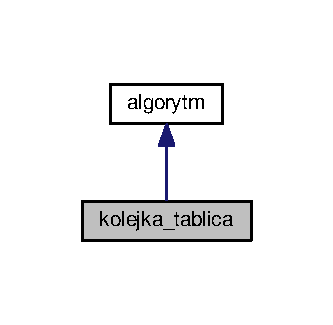
\includegraphics[width=160pt]{classkolejka__tablica__inherit__graph}
\end{center}
\end{figure}


Diagram współpracy dla kolejka\-\_\-tablica\-:\nopagebreak
\begin{figure}[H]
\begin{center}
\leavevmode
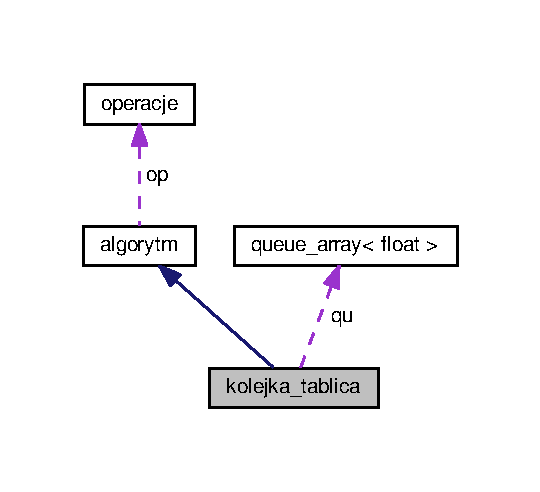
\includegraphics[width=259pt]{classkolejka__tablica__coll__graph}
\end{center}
\end{figure}
\subsection*{Metody publiczne}
\begin{DoxyCompactItemize}
\item 
\hyperlink{classkolejka__tablica_aa99b89749fcd8c780882ebbe089cad0f}{kolejka\-\_\-tablica} (ifstream \&plik1, ifstream \&plik2, int N, int M, \hyperlink{stos_8hh_a7847560c748814fd3070e9149a9578bd}{flag} F)
\begin{DoxyCompactList}\small\item\em konstruktor -\/ ustawia flage w zadany stan \end{DoxyCompactList}\item 
float \hyperlink{classkolejka__tablica_aad6baa28ce61111666e70df7d6ac4f86}{przelicz} ()
\begin{DoxyCompactList}\small\item\em Metoda odpowiada za przetworzenie danych wejsciowych zgodnie z zadanym algorytmem. \end{DoxyCompactList}\end{DoxyCompactItemize}
\subsection*{Atrybuty prywatne}
\begin{DoxyCompactItemize}
\item 
\hyperlink{classqueue__array}{queue\-\_\-array}$<$ float $>$ \hyperlink{classkolejka__tablica_a7fd15c7c7a0fa3649042ec634b2b8d4f}{qu}
\end{DoxyCompactItemize}
\subsection*{Dodatkowe Dziedziczone Składowe}


\subsection{Opis szczegółowy}
klasa utworzona na potrzeby pomiaru czasu wypełnienia struktury 

Definicja w linii 179 pliku algorytm.\-hh.



\subsection{Dokumentacja konstruktora i destruktora}
\hypertarget{classkolejka__tablica_aa99b89749fcd8c780882ebbe089cad0f}{\index{kolejka\-\_\-tablica@{kolejka\-\_\-tablica}!kolejka\-\_\-tablica@{kolejka\-\_\-tablica}}
\index{kolejka\-\_\-tablica@{kolejka\-\_\-tablica}!kolejka_tablica@{kolejka\-\_\-tablica}}
\subsubsection[{kolejka\-\_\-tablica}]{\setlength{\rightskip}{0pt plus 5cm}kolejka\-\_\-tablica\-::kolejka\-\_\-tablica (
\begin{DoxyParamCaption}
\item[{ifstream \&}]{plik1, }
\item[{ifstream \&}]{plik2, }
\item[{int}]{N, }
\item[{int}]{M, }
\item[{{\bf flag}}]{F}
\end{DoxyParamCaption}
)\hspace{0.3cm}{\ttfamily [inline]}}}\label{classkolejka__tablica_aa99b89749fcd8c780882ebbe089cad0f}


konstruktor -\/ ustawia flage w zadany stan 



Definicja w linii 185 pliku algorytm.\-hh.



\subsection{Dokumentacja funkcji składowych}
\hypertarget{classkolejka__tablica_aad6baa28ce61111666e70df7d6ac4f86}{\index{kolejka\-\_\-tablica@{kolejka\-\_\-tablica}!przelicz@{przelicz}}
\index{przelicz@{przelicz}!kolejka_tablica@{kolejka\-\_\-tablica}}
\subsubsection[{przelicz}]{\setlength{\rightskip}{0pt plus 5cm}float kolejka\-\_\-tablica\-::przelicz (
\begin{DoxyParamCaption}
{}
\end{DoxyParamCaption}
)\hspace{0.3cm}{\ttfamily [virtual]}}}\label{classkolejka__tablica_aad6baa28ce61111666e70df7d6ac4f86}


Metoda odpowiada za przetworzenie danych wejsciowych zgodnie z zadanym algorytmem. 



Reimplementowana z \hyperlink{classalgorytm_af3f92bf537b1f2e1f93173983e838449}{algorytm}.



Definicja w linii 148 pliku algorytm.\-cpp.



Oto graf wywołań dla tej funkcji\-:\nopagebreak
\begin{figure}[H]
\begin{center}
\leavevmode
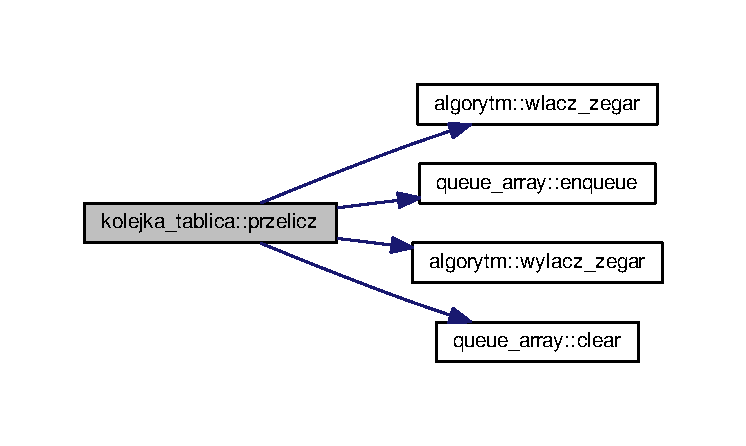
\includegraphics[width=350pt]{classkolejka__tablica_aad6baa28ce61111666e70df7d6ac4f86_cgraph}
\end{center}
\end{figure}




\subsection{Dokumentacja atrybutów składowych}
\hypertarget{classkolejka__tablica_a7fd15c7c7a0fa3649042ec634b2b8d4f}{\index{kolejka\-\_\-tablica@{kolejka\-\_\-tablica}!qu@{qu}}
\index{qu@{qu}!kolejka_tablica@{kolejka\-\_\-tablica}}
\subsubsection[{qu}]{\setlength{\rightskip}{0pt plus 5cm}{\bf queue\-\_\-array}$<$float$>$ kolejka\-\_\-tablica\-::qu\hspace{0.3cm}{\ttfamily [private]}}}\label{classkolejka__tablica_a7fd15c7c7a0fa3649042ec634b2b8d4f}


Definicja w linii 180 pliku algorytm.\-hh.



Dokumentacja dla tej klasy została wygenerowana z plików\-:\begin{DoxyCompactItemize}
\item 
\hyperlink{algorytm_8hh}{algorytm.\-hh}\item 
\hyperlink{algorytm_8cpp}{algorytm.\-cpp}\end{DoxyCompactItemize}

\hypertarget{classm__sort}{\section{\-Dokumentacja klasy m\-\_\-sort}
\label{classm__sort}\index{m\-\_\-sort@{m\-\_\-sort}}
}


klasa reprezentuje dane poddane sortowaniu przez scalanie  




{\ttfamily \#include $<$algorytm.\-hh$>$}



\-Diagram dziedziczenia dla m\-\_\-sort
\nopagebreak
\begin{figure}[H]
\begin{center}
\leavevmode
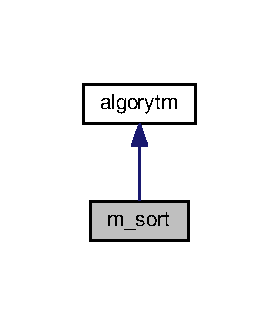
\includegraphics[width=134pt]{classm__sort__inherit__graph}
\end{center}
\end{figure}


\-Diagram współpracy dla m\-\_\-sort\-:
\nopagebreak
\begin{figure}[H]
\begin{center}
\leavevmode
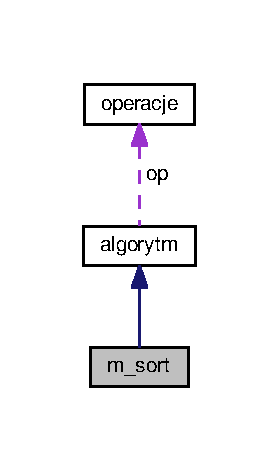
\includegraphics[width=134pt]{classm__sort__coll__graph}
\end{center}
\end{figure}
\subsection*{\-Metody publiczne}
\begin{DoxyCompactItemize}
\item 
\hyperlink{classm__sort_a9894abcd2ddd89f6963e80cc4038eed8}{m\-\_\-sort} (ifstream \&plik1, ifstream \&plik2, int \-N, int \-M)
\begin{DoxyCompactList}\small\item\em konstruktor \end{DoxyCompactList}\item 
float \hyperlink{classm__sort_acfcfa7bf26982bf718a169ccb771e694}{przelicz} ()
\begin{DoxyCompactList}\small\item\em metoda dokonujaca sortowania danych \end{DoxyCompactList}\end{DoxyCompactItemize}


\subsection{\-Opis szczegółowy}
klasa reprezentuje dane poddane sortowaniu przez scalanie 

\-Definicja w linii 212 pliku algorytm.\-hh.



\subsection{\-Dokumentacja konstruktora i destruktora}
\hypertarget{classm__sort_a9894abcd2ddd89f6963e80cc4038eed8}{\index{m\-\_\-sort@{m\-\_\-sort}!m\-\_\-sort@{m\-\_\-sort}}
\index{m\-\_\-sort@{m\-\_\-sort}!m_sort@{m\-\_\-sort}}
\subsubsection[{m\-\_\-sort}]{\setlength{\rightskip}{0pt plus 5cm}{\bf m\-\_\-sort\-::m\-\_\-sort} (
\begin{DoxyParamCaption}
\item[{ifstream \&}]{plik1, }
\item[{ifstream \&}]{plik2, }
\item[{int}]{\-N, }
\item[{int}]{\-M}
\end{DoxyParamCaption}
)\hspace{0.3cm}{\ttfamily  \mbox{[}inline\mbox{]}}}}\label{classm__sort_a9894abcd2ddd89f6963e80cc4038eed8}


konstruktor 



\-Definicja w linii 215 pliku algorytm.\-hh.



\subsection{\-Dokumentacja funkcji składowych}
\hypertarget{classm__sort_acfcfa7bf26982bf718a169ccb771e694}{\index{m\-\_\-sort@{m\-\_\-sort}!przelicz@{przelicz}}
\index{przelicz@{przelicz}!m_sort@{m\-\_\-sort}}
\subsubsection[{przelicz}]{\setlength{\rightskip}{0pt plus 5cm}float {\bf m\-\_\-sort\-::przelicz} (
\begin{DoxyParamCaption}
{}
\end{DoxyParamCaption}
)\hspace{0.3cm}{\ttfamily  \mbox{[}virtual\mbox{]}}}}\label{classm__sort_acfcfa7bf26982bf718a169ccb771e694}


metoda dokonujaca sortowania danych 



\-Reimplementowana z \hyperlink{classalgorytm_af3f92bf537b1f2e1f93173983e838449}{algorytm}.



\-Definicja w linii 183 pliku algorytm.\-cpp.



\-Oto graf wywołań dla tej funkcji\-:
\nopagebreak
\begin{figure}[H]
\begin{center}
\leavevmode
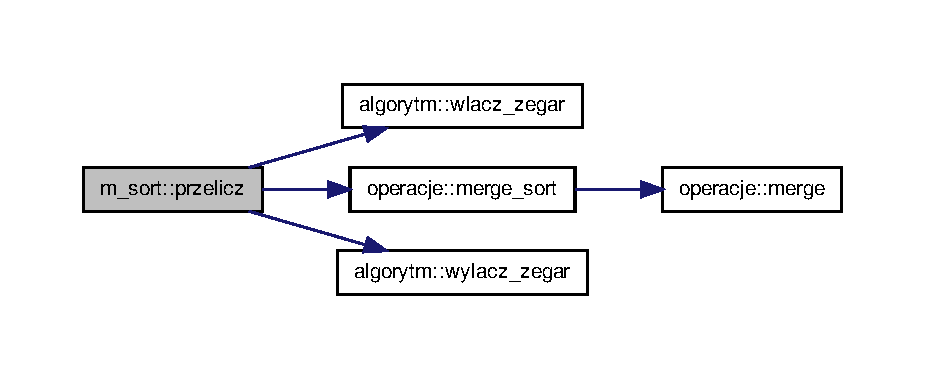
\includegraphics[width=350pt]{classm__sort_acfcfa7bf26982bf718a169ccb771e694_cgraph}
\end{center}
\end{figure}




\-Dokumentacja dla tej klasy została wygenerowana z plików\-:\begin{DoxyCompactItemize}
\item 
\hyperlink{algorytm_8hh}{algorytm.\-hh}\item 
\hyperlink{algorytm_8cpp}{algorytm.\-cpp}\end{DoxyCompactItemize}

\hypertarget{classmnozenie}{\section{\-Dokumentacja klasy mnozenie}
\label{classmnozenie}\index{mnozenie@{mnozenie}}
}


modeluje algorytm dokonujacy mnozenia kazdego elementu pliku wejsciowego przez 2  




{\ttfamily \#include $<$algorytm.\-hh$>$}



\-Diagram dziedziczenia dla mnozenie\nopagebreak
\begin{figure}[H]
\begin{center}
\leavevmode
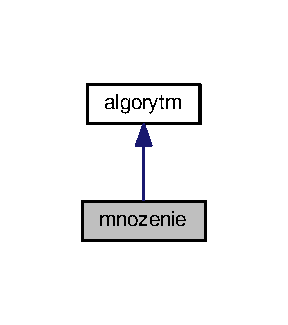
\includegraphics[width=138pt]{classmnozenie__inherit__graph}
\end{center}
\end{figure}


\-Diagram współpracy dla mnozenie\-:\nopagebreak
\begin{figure}[H]
\begin{center}
\leavevmode
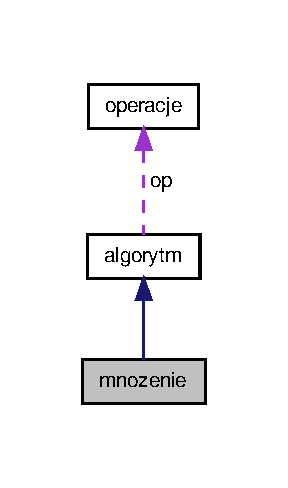
\includegraphics[width=138pt]{classmnozenie__coll__graph}
\end{center}
\end{figure}
\subsection*{\-Metody publiczne}
\begin{DoxyCompactItemize}
\item 
\hyperlink{classmnozenie_a105c483d60c621dc5c1855a04e285e3c}{mnozenie} (ifstream \&plik1, ifstream \&plik2, int \-N, int \-M)
\item 
void \hyperlink{classmnozenie_a5c97c36f9463bdf4eb7e34976a029930}{przelicz} ()
\begin{DoxyCompactList}\small\item\em wykonuje zalozony algorytm mnozenia elementow tablicy przez 2 \end{DoxyCompactList}\end{DoxyCompactItemize}


\subsection{\-Opis szczegółowy}
modeluje algorytm dokonujacy mnozenia kazdego elementu pliku wejsciowego przez 2 

\-Definicja w linii 125 pliku algorytm.\-hh.



\subsection{\-Dokumentacja konstruktora i destruktora}
\hypertarget{classmnozenie_a105c483d60c621dc5c1855a04e285e3c}{\index{mnozenie@{mnozenie}!mnozenie@{mnozenie}}
\index{mnozenie@{mnozenie}!mnozenie@{mnozenie}}
\subsubsection[{mnozenie}]{\setlength{\rightskip}{0pt plus 5cm}{\bf mnozenie\-::mnozenie} (
\begin{DoxyParamCaption}
\item[{ifstream \&}]{plik1, }
\item[{ifstream \&}]{plik2, }
\item[{int}]{\-N, }
\item[{int}]{\-M}
\end{DoxyParamCaption}
)\hspace{0.3cm}{\ttfamily  \mbox{[}inline\mbox{]}}}}\label{classmnozenie_a105c483d60c621dc5c1855a04e285e3c}
/brief konstruktor przekazuje do pol klasy informacje o nazwach pliku wejsciowego i wzorcowego 
\begin{DoxyParams}[1]{\-Parametry}
\mbox{\tt in}  & {\em plik1} & -\/ plik wejsciowy \\
\hline
\mbox{\tt in}  & {\em plik2} & -\/ plik wzorcowy \\
\hline
\mbox{\tt in}  & {\em \-N} & -\/ ilosc danych wejsciowych \\
\hline
\mbox{\tt in}  & {\em \-M} & -\/ ilosc powtorzen \\
\hline
\end{DoxyParams}


\-Definicja w linii 134 pliku algorytm.\-hh.



\subsection{\-Dokumentacja funkcji składowych}
\hypertarget{classmnozenie_a5c97c36f9463bdf4eb7e34976a029930}{\index{mnozenie@{mnozenie}!przelicz@{przelicz}}
\index{przelicz@{przelicz}!mnozenie@{mnozenie}}
\subsubsection[{przelicz}]{\setlength{\rightskip}{0pt plus 5cm}void {\bf mnozenie\-::przelicz} (
\begin{DoxyParamCaption}
{}
\end{DoxyParamCaption}
)\hspace{0.3cm}{\ttfamily  \mbox{[}virtual\mbox{]}}}}\label{classmnozenie_a5c97c36f9463bdf4eb7e34976a029930}


wykonuje zalozony algorytm mnozenia elementow tablicy przez 2 



\-Reimplementowana z \hyperlink{classalgorytm_aeefdd677ca8b9475a15547dcf8dd461f}{algorytm}.



\-Definicja w linii 81 pliku algorytm.\-cpp.



\-Dokumentacja dla tej klasy została wygenerowana z plików\-:\begin{DoxyCompactItemize}
\item 
\hyperlink{algorytm_8hh}{algorytm.\-hh}\item 
\hyperlink{algorytm_8cpp}{algorytm.\-cpp}\end{DoxyCompactItemize}

\hypertarget{classoperacje}{\section{\-Dokumentacja klasy operacje}
\label{classoperacje}\index{operacje@{operacje}}
}


\-Klasa modeluje tablice z danymi i metody sluzace do operacji na niej.  




{\ttfamily \#include $<$operacje.\-hh$>$}

\subsection*{\-Metody publiczne}
\begin{DoxyCompactItemize}
\item 
\hyperlink{classoperacje_a4538e0bfde26291449dc057134b23ad8}{operacje} ()
\begin{DoxyCompactList}\small\item\em konstruktor bezparametryczny \end{DoxyCompactList}\item 
\hyperlink{classoperacje_af109f7f9a4b10334d5e8c215c7f220de}{operacje} (int \-N)
\begin{DoxyCompactList}\small\item\em konstruktor parametryczny -\/ alokuje pamiec w dynamicznej tablicy {\ttfamily tab} \end{DoxyCompactList}\item 
bool \hyperlink{classoperacje_a7393a8b3b394921a084e0c1f4ad517b7}{zamien\-\_\-elementy} (int i, int j)
\begin{DoxyCompactList}\small\item\em \-Metoda zamienia 2 elementy tablicy. \end{DoxyCompactList}\item 
void \hyperlink{classoperacje_a7aa29c588e5a8f93c437150f03a133f1}{quick\-\_\-sort} (int l, int p)
\begin{DoxyCompactList}\small\item\em \-Metoda \-Dokonuje sortownaia szybkiego. \end{DoxyCompactList}\item 
void \hyperlink{classoperacje_a9be241905b909e7aef0151902c6f5b81}{make\-\_\-node} (int rozmiar, int i)
\begin{DoxyCompactList}\small\item\em \-Metoda tworzy wezel drzewa, przypisujac mu 2 synow, ustawiajac ich w odpowiedniej kolejnosci (ojciec ma najwieksza wartosc) \end{DoxyCompactList}\item 
void \hyperlink{classoperacje_ae752685beea6c7ee81d2347a98d40146}{make\-\_\-heap} ()
\begin{DoxyCompactList}\small\item\em \-Metoda tworzy kopiec binarny. \end{DoxyCompactList}\item 
void \hyperlink{classoperacje_aec9d2248eb072f97da794ee4c9b99a5d}{heap\-\_\-sort} ()
\begin{DoxyCompactList}\small\item\em \-Metoda dokonuje sortowania po uprzednim utworzeniu kopca. \end{DoxyCompactList}\item 
void \hyperlink{classoperacje_ad766f1d18595ff6b779485528c65d3f0}{merge} (int poczatek, int srodek, int koniec)
\begin{DoxyCompactList}\small\item\em \-Metoda scala dwie czesci tablicy, jednoczesnie je porzadkujac. \end{DoxyCompactList}\item 
void \hyperlink{classoperacje_ac65f2613b7d32b4f95e59bf2f8fd1aab}{merge\-\_\-sort} (int poczatek, int koniec)
\item 
void \hyperlink{classoperacje_aedc47c87f4f44f8af0cba64a940a5333}{odwroc\-\_\-tablice} ()
\begin{DoxyCompactList}\small\item\em metoda odwraca wszystkie elementy tablicy \end{DoxyCompactList}\item 
void \hyperlink{classoperacje_ad8397efded792c1381bfd0292b3e91b6}{dodaj\-\_\-element} (float e)
\begin{DoxyCompactList}\small\item\em metoda dodaje element do tablicy, alokujac dodatkowa pamiec \end{DoxyCompactList}\item 
void \hyperlink{classoperacje_a933533caa39434db543aca704804625c}{dodaj\-\_\-elementy} (float $\ast$tab2, int rozm)
\begin{DoxyCompactList}\small\item\em metoda dodaje elementy do tablicy \end{DoxyCompactList}\item 
void \hyperlink{classoperacje_a33127b613894949faba7a04f23075bf8}{operator=} (float $\ast$tab1)
\begin{DoxyCompactList}\small\item\em \-Przeciazenie operatora przypisania; przypisuje elementy tablicy {\ttfamily tab1} {\ttfamily do} tablicy bedacej polem klasy. \end{DoxyCompactList}\item 
bool \hyperlink{classoperacje_af69f25c4d1da5a7e46ff21a56143fc62}{operator==} (float $\ast$tab1)
\begin{DoxyCompactList}\small\item\em \-Przeciazenie operatora porownania; metoda porownuje zawartosci dwoch tablic. \end{DoxyCompactList}\item 
float \& \hyperlink{classoperacje_a6aeba674ecf3058e63e12bca9862a7fb}{operator\mbox{[}$\,$\mbox{]}} (int ind)
\end{DoxyCompactItemize}
\subsection*{\-Atrybuty publiczne}
\begin{DoxyCompactItemize}
\item 
int \hyperlink{classoperacje_aec7cc301d8822128d918aa1f9c7e1db2}{n}
\begin{DoxyCompactList}\small\item\em ilosc elementow w tablicy \end{DoxyCompactList}\item 
float $\ast$ \hyperlink{classoperacje_ad23bc418eebc9b493a5494ffd9358dd0}{tab}
\begin{DoxyCompactList}\small\item\em tablica z liczbami \end{DoxyCompactList}\end{DoxyCompactItemize}


\subsection{\-Opis szczegółowy}
\-Klasa modeluje tablice z danymi i metody sluzace do operacji na niej. 

\-Definicja w linii 11 pliku operacje.\-hh.



\subsection{\-Dokumentacja konstruktora i destruktora}
\hypertarget{classoperacje_a4538e0bfde26291449dc057134b23ad8}{\index{operacje@{operacje}!operacje@{operacje}}
\index{operacje@{operacje}!operacje@{operacje}}
\subsubsection[{operacje}]{\setlength{\rightskip}{0pt plus 5cm}{\bf operacje\-::operacje} (
\begin{DoxyParamCaption}
{}
\end{DoxyParamCaption}
)}}\label{classoperacje_a4538e0bfde26291449dc057134b23ad8}


konstruktor bezparametryczny 

\hypertarget{classoperacje_af109f7f9a4b10334d5e8c215c7f220de}{\index{operacje@{operacje}!operacje@{operacje}}
\index{operacje@{operacje}!operacje@{operacje}}
\subsubsection[{operacje}]{\setlength{\rightskip}{0pt plus 5cm}{\bf operacje\-::operacje} (
\begin{DoxyParamCaption}
\item[{int}]{\-N}
\end{DoxyParamCaption}
)\hspace{0.3cm}{\ttfamily  \mbox{[}inline\mbox{]}}}}\label{classoperacje_af109f7f9a4b10334d5e8c215c7f220de}


konstruktor parametryczny -\/ alokuje pamiec w dynamicznej tablicy {\ttfamily tab} 


\begin{DoxyParams}[1]{\-Parametry}
\mbox{\tt in}  & {\em \-N} & -\/ ilosc elementow w tablicy; parametr przypisywany do pola {\ttfamily n} w klasie, oraz alokuje pamiec o takim wlasnie rozmiarze \\
\hline
\end{DoxyParams}


\-Definicja w linii 28 pliku operacje.\-hh.



\subsection{\-Dokumentacja funkcji składowych}
\hypertarget{classoperacje_ad8397efded792c1381bfd0292b3e91b6}{\index{operacje@{operacje}!dodaj\-\_\-element@{dodaj\-\_\-element}}
\index{dodaj\-\_\-element@{dodaj\-\_\-element}!operacje@{operacje}}
\subsubsection[{dodaj\-\_\-element}]{\setlength{\rightskip}{0pt plus 5cm}void {\bf operacje\-::dodaj\-\_\-element} (
\begin{DoxyParamCaption}
\item[{float}]{e}
\end{DoxyParamCaption}
)}}\label{classoperacje_ad8397efded792c1381bfd0292b3e91b6}


metoda dodaje element do tablicy, alokujac dodatkowa pamiec 


\begin{DoxyParams}[1]{\-Parametry}
\mbox{\tt in}  & {\em e} & -\/ element, ktory nalezy dolaczyc do tablicy \\
\hline
\end{DoxyParams}


\-Definicja w linii 27 pliku operacje.\-cpp.

\hypertarget{classoperacje_a933533caa39434db543aca704804625c}{\index{operacje@{operacje}!dodaj\-\_\-elementy@{dodaj\-\_\-elementy}}
\index{dodaj\-\_\-elementy@{dodaj\-\_\-elementy}!operacje@{operacje}}
\subsubsection[{dodaj\-\_\-elementy}]{\setlength{\rightskip}{0pt plus 5cm}void {\bf operacje\-::dodaj\-\_\-elementy} (
\begin{DoxyParamCaption}
\item[{float $\ast$}]{tab2, }
\item[{int}]{rozm}
\end{DoxyParamCaption}
)}}\label{classoperacje_a933533caa39434db543aca704804625c}


metoda dodaje elementy do tablicy 


\begin{DoxyParams}[1]{\-Parametry}
\mbox{\tt in}  & {\em tab2} & -\/ tablica, ktora nalezy dolaczyc \\
\hline
\mbox{\tt in}  & {\em rozm} & -\/ rozmiar tablicy tab2 \\
\hline
\end{DoxyParams}


\-Definicja w linii 46 pliku operacje.\-cpp.

\hypertarget{classoperacje_aec9d2248eb072f97da794ee4c9b99a5d}{\index{operacje@{operacje}!heap\-\_\-sort@{heap\-\_\-sort}}
\index{heap\-\_\-sort@{heap\-\_\-sort}!operacje@{operacje}}
\subsubsection[{heap\-\_\-sort}]{\setlength{\rightskip}{0pt plus 5cm}void {\bf operacje\-::heap\-\_\-sort} (
\begin{DoxyParamCaption}
{}
\end{DoxyParamCaption}
)}}\label{classoperacje_aec9d2248eb072f97da794ee4c9b99a5d}


\-Metoda dokonuje sortowania po uprzednim utworzeniu kopca. 



\-Definicja w linii 116 pliku operacje.\-cpp.



\-Oto graf wywołań dla tej funkcji\-:\nopagebreak
\begin{figure}[H]
\begin{center}
\leavevmode
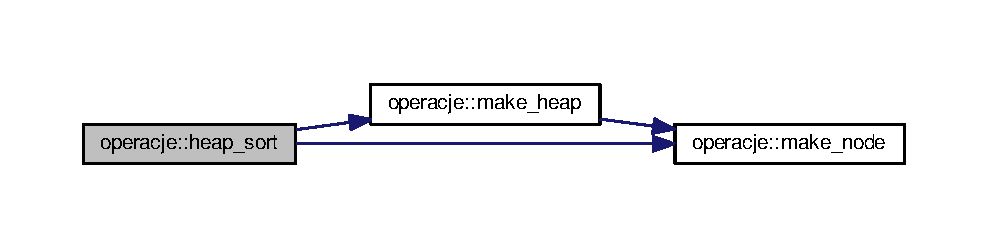
\includegraphics[width=350pt]{classoperacje_aec9d2248eb072f97da794ee4c9b99a5d_cgraph}
\end{center}
\end{figure}




\-Oto graf wywoływań tej funkcji\-:\nopagebreak
\begin{figure}[H]
\begin{center}
\leavevmode
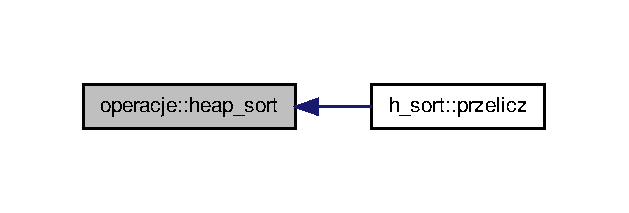
\includegraphics[width=302pt]{classoperacje_aec9d2248eb072f97da794ee4c9b99a5d_icgraph}
\end{center}
\end{figure}


\hypertarget{classoperacje_ae752685beea6c7ee81d2347a98d40146}{\index{operacje@{operacje}!make\-\_\-heap@{make\-\_\-heap}}
\index{make\-\_\-heap@{make\-\_\-heap}!operacje@{operacje}}
\subsubsection[{make\-\_\-heap}]{\setlength{\rightskip}{0pt plus 5cm}void {\bf operacje\-::make\-\_\-heap} (
\begin{DoxyParamCaption}
{}
\end{DoxyParamCaption}
)}}\label{classoperacje_ae752685beea6c7ee81d2347a98d40146}


\-Metoda tworzy kopiec binarny. 



\-Definicja w linii 110 pliku operacje.\-cpp.



\-Oto graf wywołań dla tej funkcji\-:\nopagebreak
\begin{figure}[H]
\begin{center}
\leavevmode
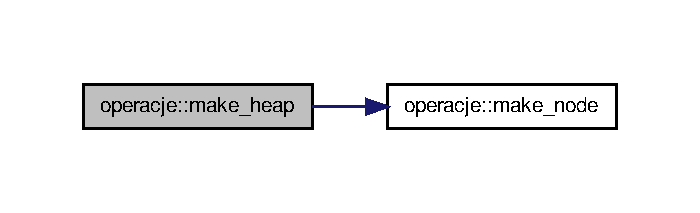
\includegraphics[width=336pt]{classoperacje_ae752685beea6c7ee81d2347a98d40146_cgraph}
\end{center}
\end{figure}




\-Oto graf wywoływań tej funkcji\-:\nopagebreak
\begin{figure}[H]
\begin{center}
\leavevmode
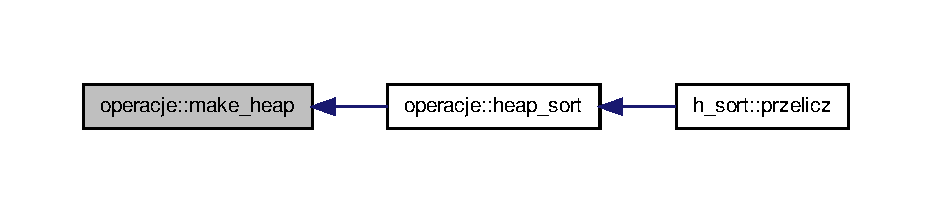
\includegraphics[width=350pt]{classoperacje_ae752685beea6c7ee81d2347a98d40146_icgraph}
\end{center}
\end{figure}


\hypertarget{classoperacje_a9be241905b909e7aef0151902c6f5b81}{\index{operacje@{operacje}!make\-\_\-node@{make\-\_\-node}}
\index{make\-\_\-node@{make\-\_\-node}!operacje@{operacje}}
\subsubsection[{make\-\_\-node}]{\setlength{\rightskip}{0pt plus 5cm}void {\bf operacje\-::make\-\_\-node} (
\begin{DoxyParamCaption}
\item[{int}]{rozmiar, }
\item[{int}]{i}
\end{DoxyParamCaption}
)}}\label{classoperacje_a9be241905b909e7aef0151902c6f5b81}


\-Metoda tworzy wezel drzewa, przypisujac mu 2 synow, ustawiajac ich w odpowiedniej kolejnosci (ojciec ma najwieksza wartosc) 


\begin{DoxyParams}[1]{\-Parametry}
\mbox{\tt in}  & {\em rozmiar} & -\/ rozmiar tablicy \\
\hline
\mbox{\tt in}  & {\em i} & -\/ indeks elementu, do ktorego przypisujemy synow \\
\hline
\end{DoxyParams}


\-Definicja w linii 95 pliku operacje.\-cpp.



\-Oto graf wywoływań tej funkcji\-:\nopagebreak
\begin{figure}[H]
\begin{center}
\leavevmode
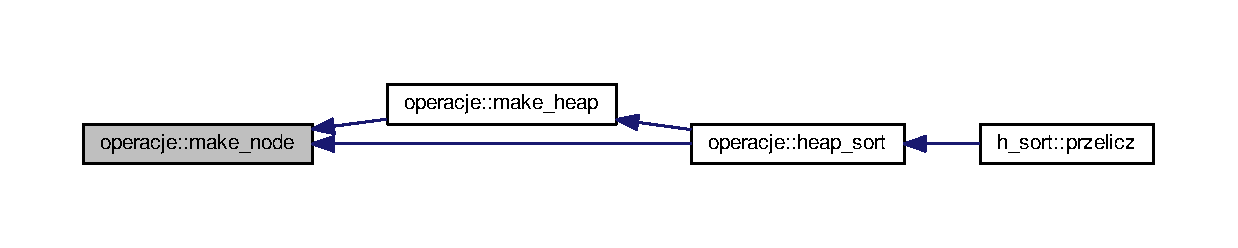
\includegraphics[width=350pt]{classoperacje_a9be241905b909e7aef0151902c6f5b81_icgraph}
\end{center}
\end{figure}


\hypertarget{classoperacje_ad766f1d18595ff6b779485528c65d3f0}{\index{operacje@{operacje}!merge@{merge}}
\index{merge@{merge}!operacje@{operacje}}
\subsubsection[{merge}]{\setlength{\rightskip}{0pt plus 5cm}void {\bf operacje\-::merge} (
\begin{DoxyParamCaption}
\item[{int}]{poczatek, }
\item[{int}]{srodek, }
\item[{int}]{koniec}
\end{DoxyParamCaption}
)}}\label{classoperacje_ad766f1d18595ff6b779485528c65d3f0}


\-Metoda scala dwie czesci tablicy, jednoczesnie je porzadkujac. 


\begin{DoxyParams}[1]{\-Parametry}
\mbox{\tt in}  & {\em poczatek} & -\/ pierwszy indeks tablicy \\
\hline
\mbox{\tt in}  & {\em srodek} & -\/ srodkowy indeks tablicy \\
\hline
\mbox{\tt in}  & {\em koniec} & -\/ ostatni indeks tablicy \\
\hline
\end{DoxyParams}


\-Definicja w linii 130 pliku operacje.\-cpp.



\-Oto graf wywoływań tej funkcji\-:\nopagebreak
\begin{figure}[H]
\begin{center}
\leavevmode
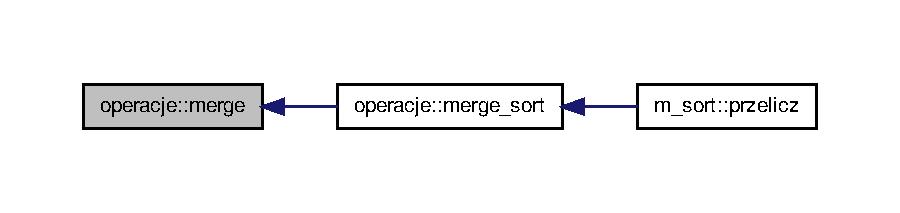
\includegraphics[width=350pt]{classoperacje_ad766f1d18595ff6b779485528c65d3f0_icgraph}
\end{center}
\end{figure}


\hypertarget{classoperacje_ac65f2613b7d32b4f95e59bf2f8fd1aab}{\index{operacje@{operacje}!merge\-\_\-sort@{merge\-\_\-sort}}
\index{merge\-\_\-sort@{merge\-\_\-sort}!operacje@{operacje}}
\subsubsection[{merge\-\_\-sort}]{\setlength{\rightskip}{0pt plus 5cm}void {\bf operacje\-::merge\-\_\-sort} (
\begin{DoxyParamCaption}
\item[{int}]{poczatek, }
\item[{int}]{koniec}
\end{DoxyParamCaption}
)}}\label{classoperacje_ac65f2613b7d32b4f95e59bf2f8fd1aab}
$\backslash$ brief \-Metoda dokonuje sortowania poprzez rekurencyjne wywolanie dla obu polow tablic, nastepnie metoda dokonuje scalenia danych 
\begin{DoxyParams}[1]{\-Parametry}
\mbox{\tt in}  & {\em poczatek} & -\/ pierwszy indeks tablicy \\
\hline
\mbox{\tt in}  & {\em koniec} & -\/ ostatni indeks tablicy \\
\hline
\end{DoxyParams}


\-Definicja w linii 166 pliku operacje.\-cpp.



\-Oto graf wywołań dla tej funkcji\-:\nopagebreak
\begin{figure}[H]
\begin{center}
\leavevmode
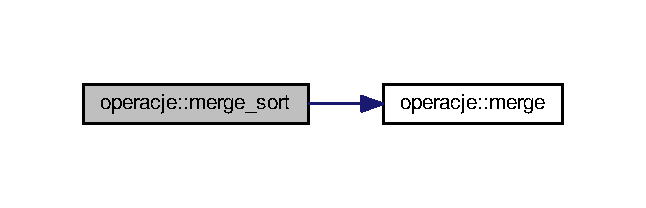
\includegraphics[width=310pt]{classoperacje_ac65f2613b7d32b4f95e59bf2f8fd1aab_cgraph}
\end{center}
\end{figure}




\-Oto graf wywoływań tej funkcji\-:\nopagebreak
\begin{figure}[H]
\begin{center}
\leavevmode
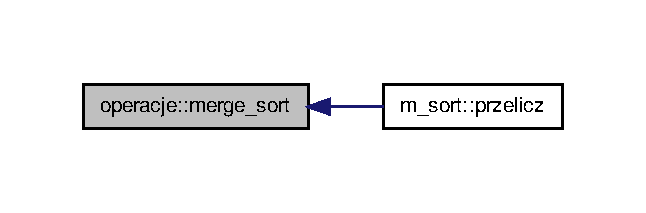
\includegraphics[width=310pt]{classoperacje_ac65f2613b7d32b4f95e59bf2f8fd1aab_icgraph}
\end{center}
\end{figure}


\hypertarget{classoperacje_aedc47c87f4f44f8af0cba64a940a5333}{\index{operacje@{operacje}!odwroc\-\_\-tablice@{odwroc\-\_\-tablice}}
\index{odwroc\-\_\-tablice@{odwroc\-\_\-tablice}!operacje@{operacje}}
\subsubsection[{odwroc\-\_\-tablice}]{\setlength{\rightskip}{0pt plus 5cm}void {\bf operacje\-::odwroc\-\_\-tablice} (
\begin{DoxyParamCaption}
{}
\end{DoxyParamCaption}
)}}\label{classoperacje_aedc47c87f4f44f8af0cba64a940a5333}


metoda odwraca wszystkie elementy tablicy 



\-Definicja w linii 12 pliku operacje.\-cpp.

\hypertarget{classoperacje_a33127b613894949faba7a04f23075bf8}{\index{operacje@{operacje}!operator=@{operator=}}
\index{operator=@{operator=}!operacje@{operacje}}
\subsubsection[{operator=}]{\setlength{\rightskip}{0pt plus 5cm}void operacje\-::operator= (
\begin{DoxyParamCaption}
\item[{float $\ast$}]{tab1}
\end{DoxyParamCaption}
)}}\label{classoperacje_a33127b613894949faba7a04f23075bf8}


\-Przeciazenie operatora przypisania; przypisuje elementy tablicy {\ttfamily tab1} {\ttfamily do} tablicy bedacej polem klasy. 


\begin{DoxyParams}[1]{\-Parametry}
\mbox{\tt in}  & {\em tab1} & -\/ tablica, ktorej zawartosc przypisujemy \\
\hline
\end{DoxyParams}


\-Definicja w linii 63 pliku operacje.\-cpp.

\hypertarget{classoperacje_af69f25c4d1da5a7e46ff21a56143fc62}{\index{operacje@{operacje}!operator==@{operator==}}
\index{operator==@{operator==}!operacje@{operacje}}
\subsubsection[{operator==}]{\setlength{\rightskip}{0pt plus 5cm}bool operacje\-::operator== (
\begin{DoxyParamCaption}
\item[{float $\ast$}]{tab1}
\end{DoxyParamCaption}
)}}\label{classoperacje_af69f25c4d1da5a7e46ff21a56143fc62}


\-Przeciazenie operatora porownania; metoda porownuje zawartosci dwoch tablic. 


\begin{DoxyParams}[1]{\-Parametry}
\mbox{\tt in}  & {\em tab1} & -\/ tablica, ktorej wartosci porownujemy \\
\hline
\end{DoxyParams}
\begin{DoxyReturn}{\-Zwraca}
true -\/ gdy zawartsoc tablic jest identyczna false -\/ w przeciwnym przypadku 
\end{DoxyReturn}


\-Definicja w linii 69 pliku operacje.\-cpp.

\hypertarget{classoperacje_a6aeba674ecf3058e63e12bca9862a7fb}{\index{operacje@{operacje}!operator\mbox{[}$\,$\mbox{]}@{operator[]}}
\index{operator\mbox{[}$\,$\mbox{]}@{operator[]}!operacje@{operacje}}
\subsubsection[{operator[]}]{\setlength{\rightskip}{0pt plus 5cm}float\& operacje\-::operator\mbox{[}$\,$\mbox{]} (
\begin{DoxyParamCaption}
\item[{int}]{ind}
\end{DoxyParamCaption}
)\hspace{0.3cm}{\ttfamily  \mbox{[}inline\mbox{]}}}}\label{classoperacje_a6aeba674ecf3058e63e12bca9862a7fb}


\-Definicja w linii 88 pliku operacje.\-hh.

\hypertarget{classoperacje_a7aa29c588e5a8f93c437150f03a133f1}{\index{operacje@{operacje}!quick\-\_\-sort@{quick\-\_\-sort}}
\index{quick\-\_\-sort@{quick\-\_\-sort}!operacje@{operacje}}
\subsubsection[{quick\-\_\-sort}]{\setlength{\rightskip}{0pt plus 5cm}void {\bf operacje\-::quick\-\_\-sort} (
\begin{DoxyParamCaption}
\item[{int}]{l, }
\item[{int}]{p}
\end{DoxyParamCaption}
)}}\label{classoperacje_a7aa29c588e5a8f93c437150f03a133f1}


\-Metoda \-Dokonuje sortownaia szybkiego. 


\begin{DoxyParams}[1]{\-Parametry}
\mbox{\tt in}  & {\em l} & -\/ pierwszy indeks tablicy \\
\hline
\mbox{\tt in}  & {\em p} & -\/ ostatni indeks tablicy \\
\hline
\end{DoxyParams}


\-Definicja w linii 77 pliku operacje.\-cpp.



\-Oto graf wywołań dla tej funkcji\-:\nopagebreak
\begin{figure}[H]
\begin{center}
\leavevmode
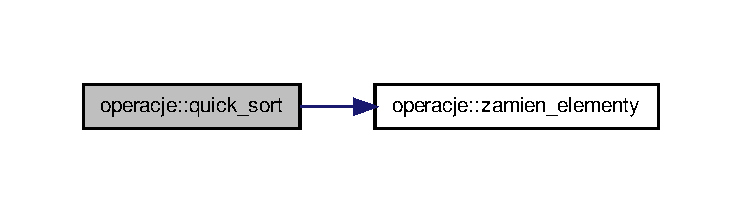
\includegraphics[width=350pt]{classoperacje_a7aa29c588e5a8f93c437150f03a133f1_cgraph}
\end{center}
\end{figure}




\-Oto graf wywoływań tej funkcji\-:\nopagebreak
\begin{figure}[H]
\begin{center}
\leavevmode
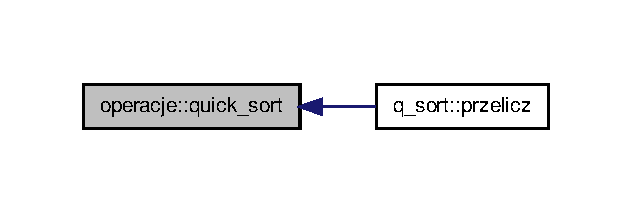
\includegraphics[width=304pt]{classoperacje_a7aa29c588e5a8f93c437150f03a133f1_icgraph}
\end{center}
\end{figure}


\hypertarget{classoperacje_a7393a8b3b394921a084e0c1f4ad517b7}{\index{operacje@{operacje}!zamien\-\_\-elementy@{zamien\-\_\-elementy}}
\index{zamien\-\_\-elementy@{zamien\-\_\-elementy}!operacje@{operacje}}
\subsubsection[{zamien\-\_\-elementy}]{\setlength{\rightskip}{0pt plus 5cm}bool {\bf operacje\-::zamien\-\_\-elementy} (
\begin{DoxyParamCaption}
\item[{int}]{i, }
\item[{int}]{j}
\end{DoxyParamCaption}
)}}\label{classoperacje_a7393a8b3b394921a084e0c1f4ad517b7}


\-Metoda zamienia 2 elementy tablicy. 


\begin{DoxyParams}[1]{\-Parametry}
\mbox{\tt in}  & {\em i} & -\/ element tablicy \\
\hline
\mbox{\tt in}  & {\em j} & -\/ element tablicy \\
\hline
\end{DoxyParams}
\begin{DoxyReturn}{\-Zwraca}
true -\/ gdy elementy nie wykraczaja poza zakres tablicy false -\/ w przeciwnym przypadku 
\end{DoxyReturn}


\-Definicja w linii 3 pliku operacje.\-cpp.



\-Oto graf wywoływań tej funkcji\-:\nopagebreak
\begin{figure}[H]
\begin{center}
\leavevmode
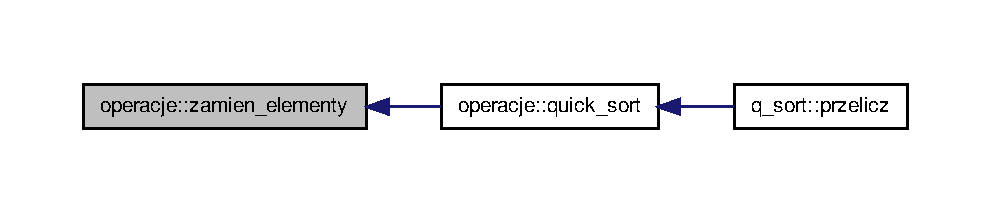
\includegraphics[width=350pt]{classoperacje_a7393a8b3b394921a084e0c1f4ad517b7_icgraph}
\end{center}
\end{figure}




\subsection{\-Dokumentacja atrybutów składowych}
\hypertarget{classoperacje_aec7cc301d8822128d918aa1f9c7e1db2}{\index{operacje@{operacje}!n@{n}}
\index{n@{n}!operacje@{operacje}}
\subsubsection[{n}]{\setlength{\rightskip}{0pt plus 5cm}int {\bf operacje\-::n}}}\label{classoperacje_aec7cc301d8822128d918aa1f9c7e1db2}


ilosc elementow w tablicy 



\-Definicja w linii 16 pliku operacje.\-hh.

\hypertarget{classoperacje_ad23bc418eebc9b493a5494ffd9358dd0}{\index{operacje@{operacje}!tab@{tab}}
\index{tab@{tab}!operacje@{operacje}}
\subsubsection[{tab}]{\setlength{\rightskip}{0pt plus 5cm}float$\ast$ {\bf operacje\-::tab}}}\label{classoperacje_ad23bc418eebc9b493a5494ffd9358dd0}


tablica z liczbami 



\-Definicja w linii 19 pliku operacje.\-hh.



\-Dokumentacja dla tej klasy została wygenerowana z plików\-:\begin{DoxyCompactItemize}
\item 
\hyperlink{operacje_8hh}{operacje.\-hh}\item 
\hyperlink{operacje_8cpp}{operacje.\-cpp}\end{DoxyCompactItemize}

\hypertarget{classq__sort}{\section{\-Dokumentacja klasy q\-\_\-sort}
\label{classq__sort}\index{q\-\_\-sort@{q\-\_\-sort}}
}


klasa reprezentuje dane poddane sortowaniu szybkiemu  




{\ttfamily \#include $<$algorytm.\-hh$>$}



\-Diagram dziedziczenia dla q\-\_\-sort
\nopagebreak
\begin{figure}[H]
\begin{center}
\leavevmode
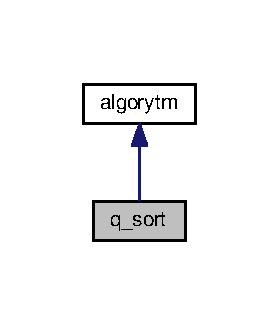
\includegraphics[width=134pt]{classq__sort__inherit__graph}
\end{center}
\end{figure}


\-Diagram współpracy dla q\-\_\-sort\-:
\nopagebreak
\begin{figure}[H]
\begin{center}
\leavevmode
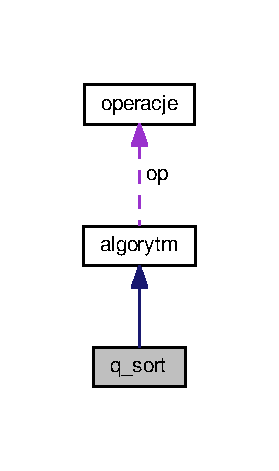
\includegraphics[width=134pt]{classq__sort__coll__graph}
\end{center}
\end{figure}
\subsection*{\-Metody publiczne}
\begin{DoxyCompactItemize}
\item 
\hyperlink{classq__sort_aeb7963f978713b880bbc19818752925d}{q\-\_\-sort} (ifstream \&plik1, ifstream \&plik2, int \-N, int \-M)
\begin{DoxyCompactList}\small\item\em konstruktor klasy \end{DoxyCompactList}\item 
float \hyperlink{classq__sort_a4f44405c764de7952fc0d821ef1206b5}{przelicz} ()
\begin{DoxyCompactList}\small\item\em metoda dokonujaca sortowania danych \end{DoxyCompactList}\end{DoxyCompactItemize}


\subsection{\-Opis szczegółowy}
klasa reprezentuje dane poddane sortowaniu szybkiemu 

\-Definicja w linii 195 pliku algorytm.\-hh.



\subsection{\-Dokumentacja konstruktora i destruktora}
\hypertarget{classq__sort_aeb7963f978713b880bbc19818752925d}{\index{q\-\_\-sort@{q\-\_\-sort}!q\-\_\-sort@{q\-\_\-sort}}
\index{q\-\_\-sort@{q\-\_\-sort}!q_sort@{q\-\_\-sort}}
\subsubsection[{q\-\_\-sort}]{\setlength{\rightskip}{0pt plus 5cm}{\bf q\-\_\-sort\-::q\-\_\-sort} (
\begin{DoxyParamCaption}
\item[{ifstream \&}]{plik1, }
\item[{ifstream \&}]{plik2, }
\item[{int}]{\-N, }
\item[{int}]{\-M}
\end{DoxyParamCaption}
)\hspace{0.3cm}{\ttfamily  \mbox{[}inline\mbox{]}}}}\label{classq__sort_aeb7963f978713b880bbc19818752925d}


konstruktor klasy 



\-Definicja w linii 198 pliku algorytm.\-hh.



\subsection{\-Dokumentacja funkcji składowych}
\hypertarget{classq__sort_a4f44405c764de7952fc0d821ef1206b5}{\index{q\-\_\-sort@{q\-\_\-sort}!przelicz@{przelicz}}
\index{przelicz@{przelicz}!q_sort@{q\-\_\-sort}}
\subsubsection[{przelicz}]{\setlength{\rightskip}{0pt plus 5cm}float {\bf q\-\_\-sort\-::przelicz} (
\begin{DoxyParamCaption}
{}
\end{DoxyParamCaption}
)\hspace{0.3cm}{\ttfamily  \mbox{[}virtual\mbox{]}}}}\label{classq__sort_a4f44405c764de7952fc0d821ef1206b5}


metoda dokonujaca sortowania danych 



\-Reimplementowana z \hyperlink{classalgorytm_af3f92bf537b1f2e1f93173983e838449}{algorytm}.



\-Definicja w linii 163 pliku algorytm.\-cpp.



\-Oto graf wywołań dla tej funkcji\-:
\nopagebreak
\begin{figure}[H]
\begin{center}
\leavevmode
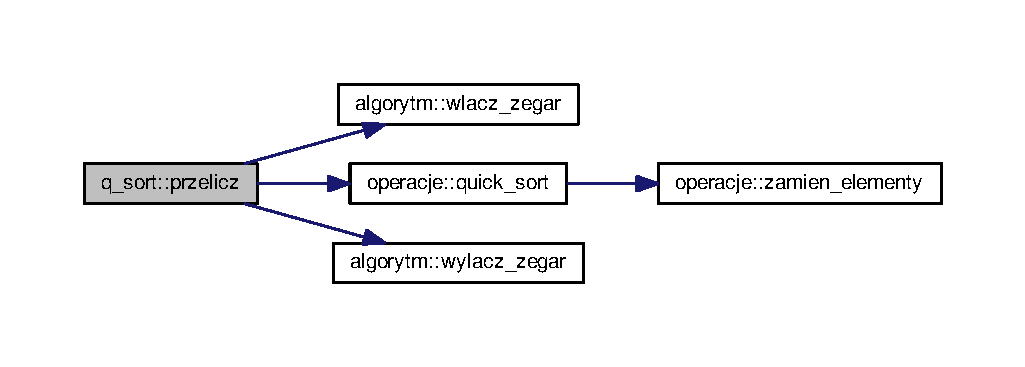
\includegraphics[width=350pt]{classq__sort_a4f44405c764de7952fc0d821ef1206b5_cgraph}
\end{center}
\end{figure}




\-Dokumentacja dla tej klasy została wygenerowana z plików\-:\begin{DoxyCompactItemize}
\item 
\hyperlink{algorytm_8hh}{algorytm.\-hh}\item 
\hyperlink{algorytm_8cpp}{algorytm.\-cpp}\end{DoxyCompactItemize}

\hypertarget{classqueue__array}{\section{Dokumentacja szablonu klasy queue\-\_\-array$<$ T\-Y\-P $>$}
\label{classqueue__array}\index{queue\-\_\-array$<$ T\-Y\-P $>$@{queue\-\_\-array$<$ T\-Y\-P $>$}}
}


Modeluje kolejke w oparciu o tablice.  




{\ttfamily \#include $<$kolejka.\-hh$>$}



Diagram współpracy dla queue\-\_\-array$<$ T\-Y\-P $>$\-:\nopagebreak
\begin{figure}[H]
\begin{center}
\leavevmode
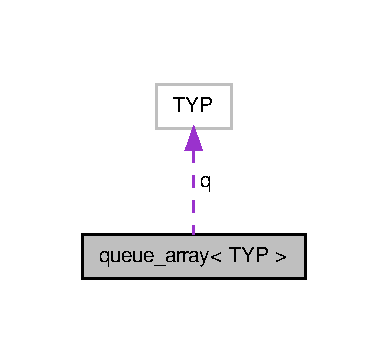
\includegraphics[width=186pt]{classqueue__array__coll__graph}
\end{center}
\end{figure}
\subsection*{Metody publiczne}
\begin{DoxyCompactItemize}
\item 
\hyperlink{classqueue__array_af651ba1c08e777af1ef23d1301819c58}{queue\-\_\-array} ()
\begin{DoxyCompactList}\small\item\em konstruktor bezparametryczny \end{DoxyCompactList}\item 
\hyperlink{classqueue__array_ad2c9f7906fad18d3daad605455210cb8}{queue\-\_\-array} (\hyperlink{stos_8hh_a7847560c748814fd3070e9149a9578bd}{flag} F)
\begin{DoxyCompactList}\small\item\em konstruktor parametryczny -\/ ustawia flage na zadana pozycje \end{DoxyCompactList}\item 
int \hyperlink{classqueue__array_a423093872e5cf4eb99f17ca1179ffa70}{size} ()
\item 
bool \hyperlink{classqueue__array_aa6ddf8e684f31a34f721e89ea83a7469}{is\-\_\-empty} ()
\item 
void \hyperlink{classqueue__array_a0c35f63c53ee3e3019fffde84bbf6bd1}{enqueue} (T\-Y\-P element)
\begin{DoxyCompactList}\small\item\em Dodaje element na poczatek kolejki w zaleznosci od wybranego trybu powiekszania tablicy. \end{DoxyCompactList}\item 
T\-Y\-P \hyperlink{classqueue__array_a67a036da416c976652c9039e5e101538}{dequeue} ()
\begin{DoxyCompactList}\small\item\em usuwa element z konca kolejki \end{DoxyCompactList}\item 
void \hyperlink{classqueue__array_acfe3b3e3ed5cc3b380d3f0d261ade3d9}{clear} ()
\begin{DoxyCompactList}\small\item\em czysci kolejke \end{DoxyCompactList}\end{DoxyCompactItemize}
\subsection*{Atrybuty publiczne}
\begin{DoxyCompactItemize}
\item 
\hyperlink{stos_8hh_a7847560c748814fd3070e9149a9578bd}{flag} \hyperlink{classqueue__array_a01c734086cf5e56c719b4d327cc36664}{f}
\begin{DoxyCompactList}\small\item\em flaga trybu zwiekszania pamieci , przyjmuje wartosc \-: plus1 -\/ dla trybu kazdorazowego powiekszania pamieci x2 -\/ dla trybu podwajania rozmiaru struktury \end{DoxyCompactList}\end{DoxyCompactItemize}
\subsection*{Atrybuty prywatne}
\begin{DoxyCompactItemize}
\item 
T\-Y\-P $\ast$ \hyperlink{classqueue__array_a073323517389c0d97534b90682317ce3}{q}
\item 
int \hyperlink{classqueue__array_a87d275726c2f69acb8ea9f0b3ab899f6}{s}
\item 
int \hyperlink{classqueue__array_a94cdc73c1df75d4fe0c75a852528cde9}{sp}
\end{DoxyCompactItemize}


\subsection{Opis szczegółowy}
\subsubsection*{template$<$typename T\-Y\-P$>$class queue\-\_\-array$<$ T\-Y\-P $>$}

Modeluje kolejke w oparciu o tablice. 

Definicja w linii 50 pliku kolejka.\-hh.



\subsection{Dokumentacja konstruktora i destruktora}
\hypertarget{classqueue__array_af651ba1c08e777af1ef23d1301819c58}{\index{queue\-\_\-array@{queue\-\_\-array}!queue\-\_\-array@{queue\-\_\-array}}
\index{queue\-\_\-array@{queue\-\_\-array}!queue_array@{queue\-\_\-array}}
\subsubsection[{queue\-\_\-array}]{\setlength{\rightskip}{0pt plus 5cm}template$<$typename T\-Y\-P$>$ {\bf queue\-\_\-array}$<$ T\-Y\-P $>$\-::{\bf queue\-\_\-array} (
\begin{DoxyParamCaption}
{}
\end{DoxyParamCaption}
)\hspace{0.3cm}{\ttfamily [inline]}}}\label{classqueue__array_af651ba1c08e777af1ef23d1301819c58}


konstruktor bezparametryczny 



Definicja w linii 63 pliku kolejka.\-hh.

\hypertarget{classqueue__array_ad2c9f7906fad18d3daad605455210cb8}{\index{queue\-\_\-array@{queue\-\_\-array}!queue\-\_\-array@{queue\-\_\-array}}
\index{queue\-\_\-array@{queue\-\_\-array}!queue_array@{queue\-\_\-array}}
\subsubsection[{queue\-\_\-array}]{\setlength{\rightskip}{0pt plus 5cm}template$<$typename T\-Y\-P$>$ {\bf queue\-\_\-array}$<$ T\-Y\-P $>$\-::{\bf queue\-\_\-array} (
\begin{DoxyParamCaption}
\item[{{\bf flag}}]{F}
\end{DoxyParamCaption}
)\hspace{0.3cm}{\ttfamily [inline]}}}\label{classqueue__array_ad2c9f7906fad18d3daad605455210cb8}


konstruktor parametryczny -\/ ustawia flage na zadana pozycje 



Definicja w linii 65 pliku kolejka.\-hh.



\subsection{Dokumentacja funkcji składowych}
\hypertarget{classqueue__array_acfe3b3e3ed5cc3b380d3f0d261ade3d9}{\index{queue\-\_\-array@{queue\-\_\-array}!clear@{clear}}
\index{clear@{clear}!queue_array@{queue\-\_\-array}}
\subsubsection[{clear}]{\setlength{\rightskip}{0pt plus 5cm}template$<$typename T\-Y\-P$>$ void {\bf queue\-\_\-array}$<$ T\-Y\-P $>$\-::clear (
\begin{DoxyParamCaption}
{}
\end{DoxyParamCaption}
)\hspace{0.3cm}{\ttfamily [inline]}}}\label{classqueue__array_acfe3b3e3ed5cc3b380d3f0d261ade3d9}


czysci kolejke 



Definicja w linii 173 pliku kolejka.\-hh.



Oto graf wywoływań tej funkcji\-:\nopagebreak
\begin{figure}[H]
\begin{center}
\leavevmode
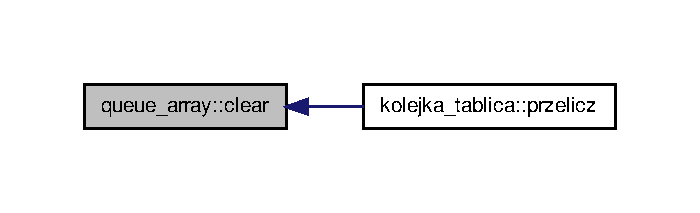
\includegraphics[width=336pt]{classqueue__array_acfe3b3e3ed5cc3b380d3f0d261ade3d9_icgraph}
\end{center}
\end{figure}


\hypertarget{classqueue__array_a67a036da416c976652c9039e5e101538}{\index{queue\-\_\-array@{queue\-\_\-array}!dequeue@{dequeue}}
\index{dequeue@{dequeue}!queue_array@{queue\-\_\-array}}
\subsubsection[{dequeue}]{\setlength{\rightskip}{0pt plus 5cm}template$<$typename T\-Y\-P$>$ T\-Y\-P {\bf queue\-\_\-array}$<$ T\-Y\-P $>$\-::dequeue (
\begin{DoxyParamCaption}
{}
\end{DoxyParamCaption}
)\hspace{0.3cm}{\ttfamily [inline]}}}\label{classqueue__array_a67a036da416c976652c9039e5e101538}


usuwa element z konca kolejki 



Definicja w linii 129 pliku kolejka.\-hh.



Oto graf wywoływań tej funkcji\-:\nopagebreak
\begin{figure}[H]
\begin{center}
\leavevmode
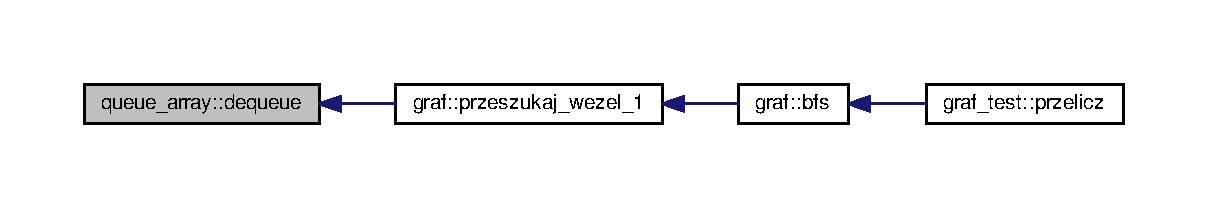
\includegraphics[width=350pt]{classqueue__array_a67a036da416c976652c9039e5e101538_icgraph}
\end{center}
\end{figure}


\hypertarget{classqueue__array_a0c35f63c53ee3e3019fffde84bbf6bd1}{\index{queue\-\_\-array@{queue\-\_\-array}!enqueue@{enqueue}}
\index{enqueue@{enqueue}!queue_array@{queue\-\_\-array}}
\subsubsection[{enqueue}]{\setlength{\rightskip}{0pt plus 5cm}template$<$typename T\-Y\-P$>$ void {\bf queue\-\_\-array}$<$ T\-Y\-P $>$\-::enqueue (
\begin{DoxyParamCaption}
\item[{T\-Y\-P}]{element}
\end{DoxyParamCaption}
)\hspace{0.3cm}{\ttfamily [inline]}}}\label{classqueue__array_a0c35f63c53ee3e3019fffde84bbf6bd1}


Dodaje element na poczatek kolejki w zaleznosci od wybranego trybu powiekszania tablicy. 



Definicja w linii 82 pliku kolejka.\-hh.



Oto graf wywoływań tej funkcji\-:\nopagebreak
\begin{figure}[H]
\begin{center}
\leavevmode
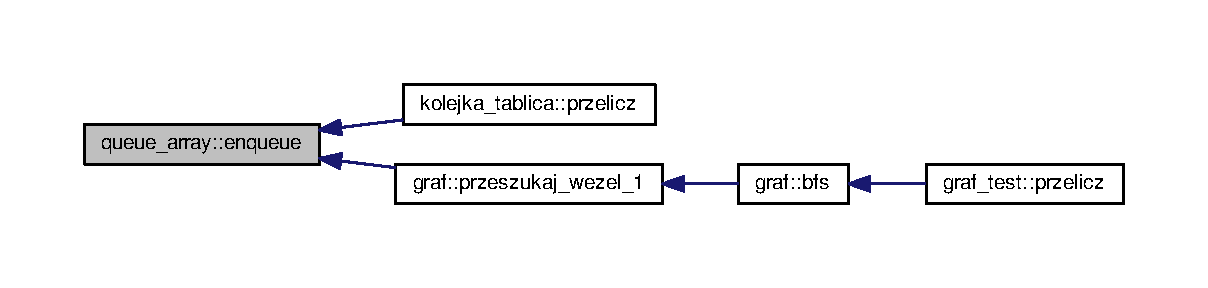
\includegraphics[width=350pt]{classqueue__array_a0c35f63c53ee3e3019fffde84bbf6bd1_icgraph}
\end{center}
\end{figure}


\hypertarget{classqueue__array_aa6ddf8e684f31a34f721e89ea83a7469}{\index{queue\-\_\-array@{queue\-\_\-array}!is\-\_\-empty@{is\-\_\-empty}}
\index{is\-\_\-empty@{is\-\_\-empty}!queue_array@{queue\-\_\-array}}
\subsubsection[{is\-\_\-empty}]{\setlength{\rightskip}{0pt plus 5cm}template$<$typename T\-Y\-P$>$ bool {\bf queue\-\_\-array}$<$ T\-Y\-P $>$\-::is\-\_\-empty (
\begin{DoxyParamCaption}
{}
\end{DoxyParamCaption}
)\hspace{0.3cm}{\ttfamily [inline]}}}\label{classqueue__array_aa6ddf8e684f31a34f721e89ea83a7469}
\begin{DoxyReturn}{Zwraca}
false -\/ gdy kolejka nie jest pusta, true , gdy pusta 
\end{DoxyReturn}


Definicja w linii 75 pliku kolejka.\-hh.



Oto graf wywoływań tej funkcji\-:\nopagebreak
\begin{figure}[H]
\begin{center}
\leavevmode
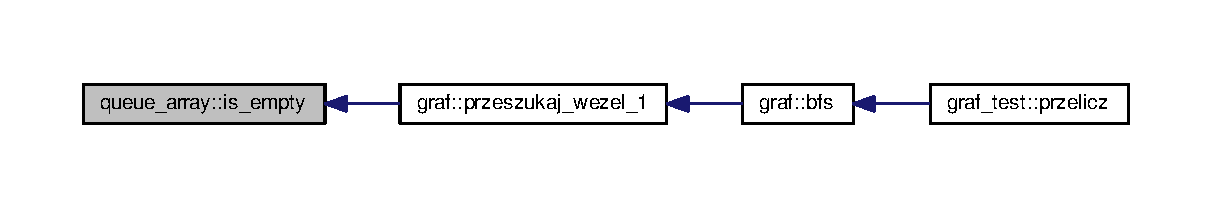
\includegraphics[width=350pt]{classqueue__array_aa6ddf8e684f31a34f721e89ea83a7469_icgraph}
\end{center}
\end{figure}


\hypertarget{classqueue__array_a423093872e5cf4eb99f17ca1179ffa70}{\index{queue\-\_\-array@{queue\-\_\-array}!size@{size}}
\index{size@{size}!queue_array@{queue\-\_\-array}}
\subsubsection[{size}]{\setlength{\rightskip}{0pt plus 5cm}template$<$typename T\-Y\-P$>$ int {\bf queue\-\_\-array}$<$ T\-Y\-P $>$\-::size (
\begin{DoxyParamCaption}
{}
\end{DoxyParamCaption}
)\hspace{0.3cm}{\ttfamily [inline]}}}\label{classqueue__array_a423093872e5cf4eb99f17ca1179ffa70}
\begin{DoxyReturn}{Zwraca}
rozmiar kolejki 
\end{DoxyReturn}


Definicja w linii 70 pliku kolejka.\-hh.



\subsection{Dokumentacja atrybutów składowych}
\hypertarget{classqueue__array_a01c734086cf5e56c719b4d327cc36664}{\index{queue\-\_\-array@{queue\-\_\-array}!f@{f}}
\index{f@{f}!queue_array@{queue\-\_\-array}}
\subsubsection[{f}]{\setlength{\rightskip}{0pt plus 5cm}template$<$typename T\-Y\-P$>$ {\bf flag} {\bf queue\-\_\-array}$<$ T\-Y\-P $>$\-::f}}\label{classqueue__array_a01c734086cf5e56c719b4d327cc36664}


flaga trybu zwiekszania pamieci , przyjmuje wartosc \-: plus1 -\/ dla trybu kazdorazowego powiekszania pamieci x2 -\/ dla trybu podwajania rozmiaru struktury 



Definicja w linii 59 pliku kolejka.\-hh.

\hypertarget{classqueue__array_a073323517389c0d97534b90682317ce3}{\index{queue\-\_\-array@{queue\-\_\-array}!q@{q}}
\index{q@{q}!queue_array@{queue\-\_\-array}}
\subsubsection[{q}]{\setlength{\rightskip}{0pt plus 5cm}template$<$typename T\-Y\-P$>$ T\-Y\-P$\ast$ {\bf queue\-\_\-array}$<$ T\-Y\-P $>$\-::q\hspace{0.3cm}{\ttfamily [private]}}}\label{classqueue__array_a073323517389c0d97534b90682317ce3}


Definicja w linii 51 pliku kolejka.\-hh.

\hypertarget{classqueue__array_a87d275726c2f69acb8ea9f0b3ab899f6}{\index{queue\-\_\-array@{queue\-\_\-array}!s@{s}}
\index{s@{s}!queue_array@{queue\-\_\-array}}
\subsubsection[{s}]{\setlength{\rightskip}{0pt plus 5cm}template$<$typename T\-Y\-P$>$ int {\bf queue\-\_\-array}$<$ T\-Y\-P $>$\-::s\hspace{0.3cm}{\ttfamily [private]}}}\label{classqueue__array_a87d275726c2f69acb8ea9f0b3ab899f6}


Definicja w linii 52 pliku kolejka.\-hh.

\hypertarget{classqueue__array_a94cdc73c1df75d4fe0c75a852528cde9}{\index{queue\-\_\-array@{queue\-\_\-array}!sp@{sp}}
\index{sp@{sp}!queue_array@{queue\-\_\-array}}
\subsubsection[{sp}]{\setlength{\rightskip}{0pt plus 5cm}template$<$typename T\-Y\-P$>$ int {\bf queue\-\_\-array}$<$ T\-Y\-P $>$\-::sp\hspace{0.3cm}{\ttfamily [private]}}}\label{classqueue__array_a94cdc73c1df75d4fe0c75a852528cde9}


Definicja w linii 52 pliku kolejka.\-hh.



Dokumentacja dla tej klasy została wygenerowana z pliku\-:\begin{DoxyCompactItemize}
\item 
\hyperlink{kolejka_8hh}{kolejka.\-hh}\end{DoxyCompactItemize}

\hypertarget{classqueue__list}{\section{\-Dokumentacja szablonu klasy queue\-\_\-list$<$ \-T\-Y\-P $>$}
\label{classqueue__list}\index{queue\-\_\-list$<$ T\-Y\-P $>$@{queue\-\_\-list$<$ T\-Y\-P $>$}}
}


\-Modeluje kolejke oparta na liscie \-S\-T\-L.  




{\ttfamily \#include $<$kolejka.\-hh$>$}

\subsection*{\-Metody publiczne}
\begin{DoxyCompactItemize}
\item 
bool \hyperlink{classqueue__list_a762d9f9f56dc9552e8df07d1b732e8b0}{is\-\_\-empty} ()
\item 
int \hyperlink{classqueue__list_aa9d1aaf18cca43fcee4e0a0dfb212cd4}{size} ()
\item 
void \hyperlink{classqueue__list_ab2985d4f0192202336311fd89d836573}{enqueue} (\-T\-Y\-P \&element)
\begin{DoxyCompactList}\small\item\em dodaje element \end{DoxyCompactList}\item 
\-T\-Y\-P \hyperlink{classqueue__list_add17ee76e80f7e09cc470ba55bd4c131}{dequeue} ()
\begin{DoxyCompactList}\small\item\em usuwa element \end{DoxyCompactList}\item 
void \hyperlink{classqueue__list_a4dcb6bb4dfee45fb084dff647ded82f0}{clear} ()
\begin{DoxyCompactList}\small\item\em czysci stos \end{DoxyCompactList}\end{DoxyCompactItemize}
\subsection*{\-Atrybuty prywatne}
\begin{DoxyCompactItemize}
\item 
list$<$ \-T\-Y\-P $>$ \hyperlink{classqueue__list_a452a11e2c4872ff7b6622d06e6d01c98}{q}
\end{DoxyCompactItemize}


\subsection{\-Opis szczegółowy}
\subsubsection*{template$<$typename \-T\-Y\-P$>$class queue\-\_\-list$<$ T\-Y\-P $>$}

\-Modeluje kolejke oparta na liscie \-S\-T\-L. 

\-Definicja w linii 19 pliku kolejka.\-hh.



\subsection{\-Dokumentacja funkcji składowych}
\hypertarget{classqueue__list_a4dcb6bb4dfee45fb084dff647ded82f0}{\index{queue\-\_\-list@{queue\-\_\-list}!clear@{clear}}
\index{clear@{clear}!queue_list@{queue\-\_\-list}}
\subsubsection[{clear}]{\setlength{\rightskip}{0pt plus 5cm}template$<$typename \-T\-Y\-P$>$ void {\bf queue\-\_\-list}$<$ \-T\-Y\-P $>$\-::{\bf clear} (
\begin{DoxyParamCaption}
{}
\end{DoxyParamCaption}
)\hspace{0.3cm}{\ttfamily  \mbox{[}inline\mbox{]}}}}\label{classqueue__list_a4dcb6bb4dfee45fb084dff647ded82f0}


czysci stos 



\-Definicja w linii 41 pliku kolejka.\-hh.



\-Oto graf wywoływań tej funkcji\-:\nopagebreak
\begin{figure}[H]
\begin{center}
\leavevmode
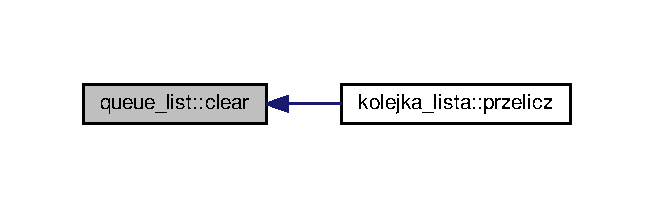
\includegraphics[width=314pt]{classqueue__list_a4dcb6bb4dfee45fb084dff647ded82f0_icgraph}
\end{center}
\end{figure}


\hypertarget{classqueue__list_add17ee76e80f7e09cc470ba55bd4c131}{\index{queue\-\_\-list@{queue\-\_\-list}!dequeue@{dequeue}}
\index{dequeue@{dequeue}!queue_list@{queue\-\_\-list}}
\subsubsection[{dequeue}]{\setlength{\rightskip}{0pt plus 5cm}template$<$typename \-T\-Y\-P$>$ \-T\-Y\-P {\bf queue\-\_\-list}$<$ \-T\-Y\-P $>$\-::{\bf dequeue} (
\begin{DoxyParamCaption}
{}
\end{DoxyParamCaption}
)\hspace{0.3cm}{\ttfamily  \mbox{[}inline\mbox{]}}}}\label{classqueue__list_add17ee76e80f7e09cc470ba55bd4c131}


usuwa element 



\-Definicja w linii 35 pliku kolejka.\-hh.

\hypertarget{classqueue__list_ab2985d4f0192202336311fd89d836573}{\index{queue\-\_\-list@{queue\-\_\-list}!enqueue@{enqueue}}
\index{enqueue@{enqueue}!queue_list@{queue\-\_\-list}}
\subsubsection[{enqueue}]{\setlength{\rightskip}{0pt plus 5cm}template$<$typename \-T\-Y\-P$>$ void {\bf queue\-\_\-list}$<$ \-T\-Y\-P $>$\-::{\bf enqueue} (
\begin{DoxyParamCaption}
\item[{\-T\-Y\-P \&}]{element}
\end{DoxyParamCaption}
)\hspace{0.3cm}{\ttfamily  \mbox{[}inline\mbox{]}}}}\label{classqueue__list_ab2985d4f0192202336311fd89d836573}


dodaje element 



\-Definicja w linii 33 pliku kolejka.\-hh.



\-Oto graf wywoływań tej funkcji\-:\nopagebreak
\begin{figure}[H]
\begin{center}
\leavevmode
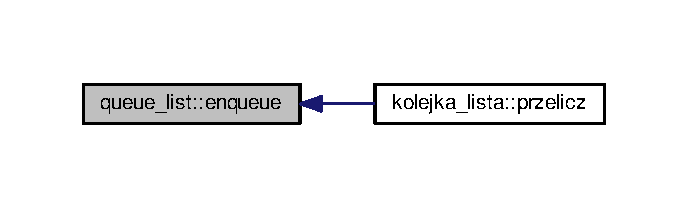
\includegraphics[width=330pt]{classqueue__list_ab2985d4f0192202336311fd89d836573_icgraph}
\end{center}
\end{figure}


\hypertarget{classqueue__list_a762d9f9f56dc9552e8df07d1b732e8b0}{\index{queue\-\_\-list@{queue\-\_\-list}!is\-\_\-empty@{is\-\_\-empty}}
\index{is\-\_\-empty@{is\-\_\-empty}!queue_list@{queue\-\_\-list}}
\subsubsection[{is\-\_\-empty}]{\setlength{\rightskip}{0pt plus 5cm}template$<$typename \-T\-Y\-P$>$ bool {\bf queue\-\_\-list}$<$ \-T\-Y\-P $>$\-::{\bf is\-\_\-empty} (
\begin{DoxyParamCaption}
{}
\end{DoxyParamCaption}
)\hspace{0.3cm}{\ttfamily  \mbox{[}inline\mbox{]}}}}\label{classqueue__list_a762d9f9f56dc9552e8df07d1b732e8b0}
\begin{DoxyReturn}{\-Zwraca}
false -\/ gdy kolejka nie jest pusta, true , gdy pusta 
\end{DoxyReturn}


\-Definicja w linii 26 pliku kolejka.\-hh.

\hypertarget{classqueue__list_aa9d1aaf18cca43fcee4e0a0dfb212cd4}{\index{queue\-\_\-list@{queue\-\_\-list}!size@{size}}
\index{size@{size}!queue_list@{queue\-\_\-list}}
\subsubsection[{size}]{\setlength{\rightskip}{0pt plus 5cm}template$<$typename \-T\-Y\-P$>$ int {\bf queue\-\_\-list}$<$ \-T\-Y\-P $>$\-::{\bf size} (
\begin{DoxyParamCaption}
{}
\end{DoxyParamCaption}
)\hspace{0.3cm}{\ttfamily  \mbox{[}inline\mbox{]}}}}\label{classqueue__list_aa9d1aaf18cca43fcee4e0a0dfb212cd4}
\begin{DoxyReturn}{\-Zwraca}
rozmiar kolejki 
\end{DoxyReturn}


\-Definicja w linii 31 pliku kolejka.\-hh.



\subsection{\-Dokumentacja atrybutów składowych}
\hypertarget{classqueue__list_a452a11e2c4872ff7b6622d06e6d01c98}{\index{queue\-\_\-list@{queue\-\_\-list}!q@{q}}
\index{q@{q}!queue_list@{queue\-\_\-list}}
\subsubsection[{q}]{\setlength{\rightskip}{0pt plus 5cm}template$<$typename \-T\-Y\-P$>$ list$<$\-T\-Y\-P$>$ {\bf queue\-\_\-list}$<$ \-T\-Y\-P $>$\-::{\bf q}\hspace{0.3cm}{\ttfamily  \mbox{[}private\mbox{]}}}}\label{classqueue__list_a452a11e2c4872ff7b6622d06e6d01c98}


\-Definicja w linii 20 pliku kolejka.\-hh.



\-Dokumentacja dla tej klasy została wygenerowana z pliku\-:\begin{DoxyCompactItemize}
\item 
\hyperlink{kolejka_8hh}{kolejka.\-hh}\end{DoxyCompactItemize}

\hypertarget{classstack__array}{\section{\-Dokumentacja szablonu klasy stack\-\_\-array$<$ \-T\-Y\-P $>$}
\label{classstack__array}\index{stack\-\_\-array$<$ T\-Y\-P $>$@{stack\-\_\-array$<$ T\-Y\-P $>$}}
}


\-Modeluje stos w oparciu o tablice.  




{\ttfamily \#include $<$stos.\-hh$>$}



\-Diagram współpracy dla stack\-\_\-array$<$ \-T\-Y\-P $>$\-:\nopagebreak
\begin{figure}[H]
\begin{center}
\leavevmode
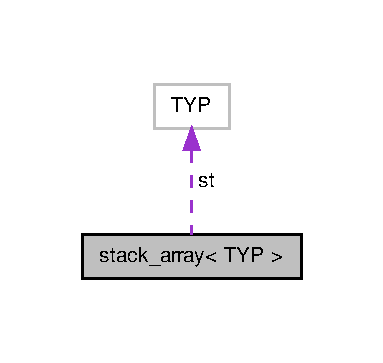
\includegraphics[width=184pt]{classstack__array__coll__graph}
\end{center}
\end{figure}
\subsection*{\-Metody publiczne}
\begin{DoxyCompactItemize}
\item 
\hyperlink{classstack__array_a430ec07ba59152bdb618039ae5f74482}{stack\-\_\-array} ()
\begin{DoxyCompactList}\small\item\em konstruktor bezparametryczny \end{DoxyCompactList}\item 
\hyperlink{classstack__array_ad6ac30696a594fc1f4b58cc94facad9f}{stack\-\_\-array} (\hyperlink{stos_8hh_a7847560c748814fd3070e9149a9578bd}{flag} \-F)
\begin{DoxyCompactList}\small\item\em konstruktor parametryczny -\/ ustawia flage na zadana pozycje \end{DoxyCompactList}\item 
bool \hyperlink{classstack__array_a653b67eb0566e9481e3525dd2f2bc519}{is\-\_\-empty} ()
\item 
int \hyperlink{classstack__array_a26ee4c653f299d3fe03b443f6180d745}{size} ()
\item 
void \hyperlink{classstack__array_a2f48529c5e88d82f5da2b27c945e1b0e}{push} (\-T\-Y\-P \&element)
\begin{DoxyCompactList}\small\item\em \-Dodaje element na wierzch stosu w zaleznosci od wybranego trybu powiekszania tablicy. \end{DoxyCompactList}\item 
\-T\-Y\-P \hyperlink{classstack__array_ad2ce52b1a99f72d383b429dff262b9eb}{pop} ()
\begin{DoxyCompactList}\small\item\em zdejmuje element ze stosu \end{DoxyCompactList}\item 
void \hyperlink{classstack__array_ac55f6fe35d44781d918884e4c466d3ee}{clear} ()
\begin{DoxyCompactList}\small\item\em czysci stos \end{DoxyCompactList}\end{DoxyCompactItemize}
\subsection*{\-Atrybuty publiczne}
\begin{DoxyCompactItemize}
\item 
\hyperlink{stos_8hh_a7847560c748814fd3070e9149a9578bd}{flag} \hyperlink{classstack__array_a06357855e64616369e11f330191413ee}{f}
\begin{DoxyCompactList}\small\item\em flaga trybu zwiekszania pamieci , przyjmuje wartosc \-: \par
 plus1 -\/ dla trybu kazdorazowego powiekszania pamieci \par
 x2 -\/ dla trybu podwajania rozmiaru struktury \end{DoxyCompactList}\end{DoxyCompactItemize}
\subsection*{\-Atrybuty prywatne}
\begin{DoxyCompactItemize}
\item 
\-T\-Y\-P $\ast$ \hyperlink{classstack__array_aa97b399041c2d08b3955bb6436cbcf2f}{st}
\item 
int \hyperlink{classstack__array_aa5730e580f60bd7b7ba77d762703fbc6}{s}
\item 
int \hyperlink{classstack__array_a598f4974aca293a20a809788ffe80b15}{sp}
\end{DoxyCompactItemize}


\subsection{\-Opis szczegółowy}
\subsubsection*{template$<$typename \-T\-Y\-P$>$class stack\-\_\-array$<$ T\-Y\-P $>$}

\-Modeluje stos w oparciu o tablice. 

\-Definicja w linii 59 pliku stos.\-hh.



\subsection{\-Dokumentacja konstruktora i destruktora}
\hypertarget{classstack__array_a430ec07ba59152bdb618039ae5f74482}{\index{stack\-\_\-array@{stack\-\_\-array}!stack\-\_\-array@{stack\-\_\-array}}
\index{stack\-\_\-array@{stack\-\_\-array}!stack_array@{stack\-\_\-array}}
\subsubsection[{stack\-\_\-array}]{\setlength{\rightskip}{0pt plus 5cm}template$<$typename \-T\-Y\-P$>$ {\bf stack\-\_\-array}$<$ \-T\-Y\-P $>$\-::{\bf stack\-\_\-array} (
\begin{DoxyParamCaption}
{}
\end{DoxyParamCaption}
)\hspace{0.3cm}{\ttfamily  \mbox{[}inline\mbox{]}}}}\label{classstack__array_a430ec07ba59152bdb618039ae5f74482}


konstruktor bezparametryczny 



\-Definicja w linii 72 pliku stos.\-hh.

\hypertarget{classstack__array_ad6ac30696a594fc1f4b58cc94facad9f}{\index{stack\-\_\-array@{stack\-\_\-array}!stack\-\_\-array@{stack\-\_\-array}}
\index{stack\-\_\-array@{stack\-\_\-array}!stack_array@{stack\-\_\-array}}
\subsubsection[{stack\-\_\-array}]{\setlength{\rightskip}{0pt plus 5cm}template$<$typename \-T\-Y\-P$>$ {\bf stack\-\_\-array}$<$ \-T\-Y\-P $>$\-::{\bf stack\-\_\-array} (
\begin{DoxyParamCaption}
\item[{{\bf flag}}]{\-F}
\end{DoxyParamCaption}
)\hspace{0.3cm}{\ttfamily  \mbox{[}inline\mbox{]}}}}\label{classstack__array_ad6ac30696a594fc1f4b58cc94facad9f}


konstruktor parametryczny -\/ ustawia flage na zadana pozycje 



\-Definicja w linii 74 pliku stos.\-hh.



\subsection{\-Dokumentacja funkcji składowych}
\hypertarget{classstack__array_ac55f6fe35d44781d918884e4c466d3ee}{\index{stack\-\_\-array@{stack\-\_\-array}!clear@{clear}}
\index{clear@{clear}!stack_array@{stack\-\_\-array}}
\subsubsection[{clear}]{\setlength{\rightskip}{0pt plus 5cm}template$<$typename \-T\-Y\-P$>$ void {\bf stack\-\_\-array}$<$ \-T\-Y\-P $>$\-::{\bf clear} (
\begin{DoxyParamCaption}
{}
\end{DoxyParamCaption}
)\hspace{0.3cm}{\ttfamily  \mbox{[}inline\mbox{]}}}}\label{classstack__array_ac55f6fe35d44781d918884e4c466d3ee}


czysci stos 



\-Definicja w linii 178 pliku stos.\-hh.



\-Oto graf wywoływań tej funkcji\-:\nopagebreak
\begin{figure}[H]
\begin{center}
\leavevmode
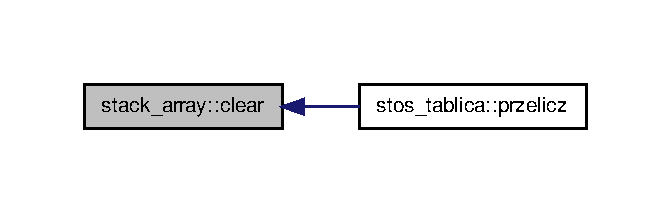
\includegraphics[width=322pt]{classstack__array_ac55f6fe35d44781d918884e4c466d3ee_icgraph}
\end{center}
\end{figure}


\hypertarget{classstack__array_a653b67eb0566e9481e3525dd2f2bc519}{\index{stack\-\_\-array@{stack\-\_\-array}!is\-\_\-empty@{is\-\_\-empty}}
\index{is\-\_\-empty@{is\-\_\-empty}!stack_array@{stack\-\_\-array}}
\subsubsection[{is\-\_\-empty}]{\setlength{\rightskip}{0pt plus 5cm}template$<$typename \-T\-Y\-P$>$ bool {\bf stack\-\_\-array}$<$ \-T\-Y\-P $>$\-::{\bf is\-\_\-empty} (
\begin{DoxyParamCaption}
{}
\end{DoxyParamCaption}
)\hspace{0.3cm}{\ttfamily  \mbox{[}inline\mbox{]}}}}\label{classstack__array_a653b67eb0566e9481e3525dd2f2bc519}
\begin{DoxyReturn}{\-Zwraca}
false -\/ gdy stos nie jest pusty, true , gdy pusty 
\end{DoxyReturn}


\-Definicja w linii 79 pliku stos.\-hh.

\hypertarget{classstack__array_ad2ce52b1a99f72d383b429dff262b9eb}{\index{stack\-\_\-array@{stack\-\_\-array}!pop@{pop}}
\index{pop@{pop}!stack_array@{stack\-\_\-array}}
\subsubsection[{pop}]{\setlength{\rightskip}{0pt plus 5cm}template$<$typename \-T\-Y\-P$>$ \-T\-Y\-P {\bf stack\-\_\-array}$<$ \-T\-Y\-P $>$\-::{\bf pop} (
\begin{DoxyParamCaption}
{}
\end{DoxyParamCaption}
)\hspace{0.3cm}{\ttfamily  \mbox{[}inline\mbox{]}}}}\label{classstack__array_ad2ce52b1a99f72d383b429dff262b9eb}


zdejmuje element ze stosu 



\-Definicja w linii 135 pliku stos.\-hh.

\hypertarget{classstack__array_a2f48529c5e88d82f5da2b27c945e1b0e}{\index{stack\-\_\-array@{stack\-\_\-array}!push@{push}}
\index{push@{push}!stack_array@{stack\-\_\-array}}
\subsubsection[{push}]{\setlength{\rightskip}{0pt plus 5cm}template$<$typename \-T\-Y\-P$>$ void {\bf stack\-\_\-array}$<$ \-T\-Y\-P $>$\-::{\bf push} (
\begin{DoxyParamCaption}
\item[{\-T\-Y\-P \&}]{element}
\end{DoxyParamCaption}
)\hspace{0.3cm}{\ttfamily  \mbox{[}inline\mbox{]}}}}\label{classstack__array_a2f48529c5e88d82f5da2b27c945e1b0e}


\-Dodaje element na wierzch stosu w zaleznosci od wybranego trybu powiekszania tablicy. 



\-Definicja w linii 91 pliku stos.\-hh.



\-Oto graf wywoływań tej funkcji\-:\nopagebreak
\begin{figure}[H]
\begin{center}
\leavevmode
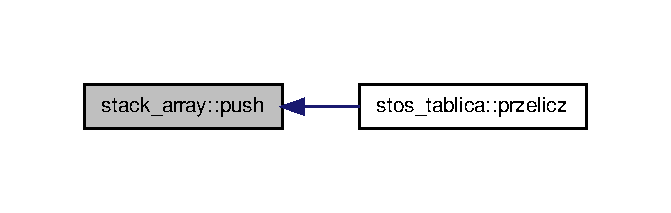
\includegraphics[width=322pt]{classstack__array_a2f48529c5e88d82f5da2b27c945e1b0e_icgraph}
\end{center}
\end{figure}


\hypertarget{classstack__array_a26ee4c653f299d3fe03b443f6180d745}{\index{stack\-\_\-array@{stack\-\_\-array}!size@{size}}
\index{size@{size}!stack_array@{stack\-\_\-array}}
\subsubsection[{size}]{\setlength{\rightskip}{0pt plus 5cm}template$<$typename \-T\-Y\-P$>$ int {\bf stack\-\_\-array}$<$ \-T\-Y\-P $>$\-::{\bf size} (
\begin{DoxyParamCaption}
{}
\end{DoxyParamCaption}
)\hspace{0.3cm}{\ttfamily  \mbox{[}inline\mbox{]}}}}\label{classstack__array_a26ee4c653f299d3fe03b443f6180d745}
\begin{DoxyReturn}{\-Zwraca}
rozmiar ztosu 
\end{DoxyReturn}


\-Definicja w linii 87 pliku stos.\-hh.



\subsection{\-Dokumentacja atrybutów składowych}
\hypertarget{classstack__array_a06357855e64616369e11f330191413ee}{\index{stack\-\_\-array@{stack\-\_\-array}!f@{f}}
\index{f@{f}!stack_array@{stack\-\_\-array}}
\subsubsection[{f}]{\setlength{\rightskip}{0pt plus 5cm}template$<$typename \-T\-Y\-P$>$ {\bf flag} {\bf stack\-\_\-array}$<$ \-T\-Y\-P $>$\-::{\bf f}}}\label{classstack__array_a06357855e64616369e11f330191413ee}


flaga trybu zwiekszania pamieci , przyjmuje wartosc \-: \par
 plus1 -\/ dla trybu kazdorazowego powiekszania pamieci \par
 x2 -\/ dla trybu podwajania rozmiaru struktury 



\-Definicja w linii 68 pliku stos.\-hh.

\hypertarget{classstack__array_aa5730e580f60bd7b7ba77d762703fbc6}{\index{stack\-\_\-array@{stack\-\_\-array}!s@{s}}
\index{s@{s}!stack_array@{stack\-\_\-array}}
\subsubsection[{s}]{\setlength{\rightskip}{0pt plus 5cm}template$<$typename \-T\-Y\-P$>$ int {\bf stack\-\_\-array}$<$ \-T\-Y\-P $>$\-::{\bf s}\hspace{0.3cm}{\ttfamily  \mbox{[}private\mbox{]}}}}\label{classstack__array_aa5730e580f60bd7b7ba77d762703fbc6}


\-Definicja w linii 61 pliku stos.\-hh.

\hypertarget{classstack__array_a598f4974aca293a20a809788ffe80b15}{\index{stack\-\_\-array@{stack\-\_\-array}!sp@{sp}}
\index{sp@{sp}!stack_array@{stack\-\_\-array}}
\subsubsection[{sp}]{\setlength{\rightskip}{0pt plus 5cm}template$<$typename \-T\-Y\-P$>$ int {\bf stack\-\_\-array}$<$ \-T\-Y\-P $>$\-::{\bf sp}\hspace{0.3cm}{\ttfamily  \mbox{[}private\mbox{]}}}}\label{classstack__array_a598f4974aca293a20a809788ffe80b15}


\-Definicja w linii 61 pliku stos.\-hh.

\hypertarget{classstack__array_aa97b399041c2d08b3955bb6436cbcf2f}{\index{stack\-\_\-array@{stack\-\_\-array}!st@{st}}
\index{st@{st}!stack_array@{stack\-\_\-array}}
\subsubsection[{st}]{\setlength{\rightskip}{0pt plus 5cm}template$<$typename \-T\-Y\-P$>$ \-T\-Y\-P$\ast$ {\bf stack\-\_\-array}$<$ \-T\-Y\-P $>$\-::{\bf st}\hspace{0.3cm}{\ttfamily  \mbox{[}private\mbox{]}}}}\label{classstack__array_aa97b399041c2d08b3955bb6436cbcf2f}


\-Definicja w linii 60 pliku stos.\-hh.



\-Dokumentacja dla tej klasy została wygenerowana z pliku\-:\begin{DoxyCompactItemize}
\item 
\hyperlink{stos_8hh}{stos.\-hh}\end{DoxyCompactItemize}

\hypertarget{classstack__list}{\section{Dokumentacja szablonu klasy stack\-\_\-list$<$ T\-Y\-P $>$}
\label{classstack__list}\index{stack\-\_\-list$<$ T\-Y\-P $>$@{stack\-\_\-list$<$ T\-Y\-P $>$}}
}


Modeluje stos oparty na liscie S\-T\-L.  




{\ttfamily \#include $<$stos.\-hh$>$}

\subsection*{Metody publiczne}
\begin{DoxyCompactItemize}
\item 
bool \hyperlink{classstack__list_a7f01744a7674ca41f55f2ea782360215}{is\-\_\-empty} ()
\item 
int \hyperlink{classstack__list_adcb1450ccbd547750e6a7939984a7c44}{size} ()
\item 
void \hyperlink{classstack__list_a7c8c94a164f180c87fa1d7a8be146a4c}{push} (T\-Y\-P \&element)
\begin{DoxyCompactList}\small\item\em Dodaje element na wierzch stosu. \end{DoxyCompactList}\item 
T\-Y\-P \hyperlink{classstack__list_aa77f6e528341ca41aefec405ebe6cd4f}{pop} ()
\begin{DoxyCompactList}\small\item\em zdejmuje element z wierzchu stosu \end{DoxyCompactList}\item 
void \hyperlink{classstack__list_afb284368d44ea1f2ab231c8f662deb5f}{clear} ()
\begin{DoxyCompactList}\small\item\em czysci stos \end{DoxyCompactList}\end{DoxyCompactItemize}
\subsection*{Atrybuty prywatne}
\begin{DoxyCompactItemize}
\item 
list$<$ T\-Y\-P $>$ \hyperlink{classstack__list_a3689c3e1f740bb83ec4471f0487a78a9}{st}
\end{DoxyCompactItemize}


\subsection{Opis szczegółowy}
\subsubsection*{template$<$typename T\-Y\-P$>$class stack\-\_\-list$<$ T\-Y\-P $>$}

Modeluje stos oparty na liscie S\-T\-L. 

Definicja w linii 22 pliku stos.\-hh.



\subsection{Dokumentacja funkcji składowych}
\hypertarget{classstack__list_afb284368d44ea1f2ab231c8f662deb5f}{\index{stack\-\_\-list@{stack\-\_\-list}!clear@{clear}}
\index{clear@{clear}!stack_list@{stack\-\_\-list}}
\subsubsection[{clear}]{\setlength{\rightskip}{0pt plus 5cm}template$<$typename T\-Y\-P$>$ void {\bf stack\-\_\-list}$<$ T\-Y\-P $>$\-::clear (
\begin{DoxyParamCaption}
{}
\end{DoxyParamCaption}
)\hspace{0.3cm}{\ttfamily [inline]}}}\label{classstack__list_afb284368d44ea1f2ab231c8f662deb5f}


czysci stos 



Definicja w linii 50 pliku stos.\-hh.



Oto graf wywoływań tej funkcji\-:\nopagebreak
\begin{figure}[H]
\begin{center}
\leavevmode
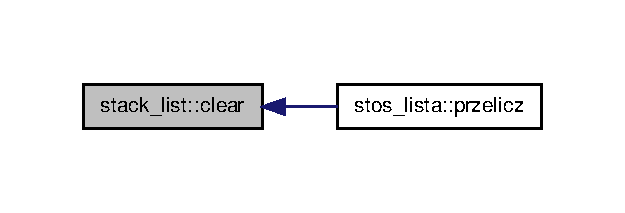
\includegraphics[width=300pt]{classstack__list_afb284368d44ea1f2ab231c8f662deb5f_icgraph}
\end{center}
\end{figure}


\hypertarget{classstack__list_a7f01744a7674ca41f55f2ea782360215}{\index{stack\-\_\-list@{stack\-\_\-list}!is\-\_\-empty@{is\-\_\-empty}}
\index{is\-\_\-empty@{is\-\_\-empty}!stack_list@{stack\-\_\-list}}
\subsubsection[{is\-\_\-empty}]{\setlength{\rightskip}{0pt plus 5cm}template$<$typename T\-Y\-P$>$ bool {\bf stack\-\_\-list}$<$ T\-Y\-P $>$\-::is\-\_\-empty (
\begin{DoxyParamCaption}
{}
\end{DoxyParamCaption}
)\hspace{0.3cm}{\ttfamily [inline]}}}\label{classstack__list_a7f01744a7674ca41f55f2ea782360215}
\begin{DoxyReturn}{Zwraca}
false -\/ gdy stos nie jest pusty, true , gdy pusty 
\end{DoxyReturn}


Definicja w linii 29 pliku stos.\-hh.

\hypertarget{classstack__list_aa77f6e528341ca41aefec405ebe6cd4f}{\index{stack\-\_\-list@{stack\-\_\-list}!pop@{pop}}
\index{pop@{pop}!stack_list@{stack\-\_\-list}}
\subsubsection[{pop}]{\setlength{\rightskip}{0pt plus 5cm}template$<$typename T\-Y\-P$>$ T\-Y\-P {\bf stack\-\_\-list}$<$ T\-Y\-P $>$\-::pop (
\begin{DoxyParamCaption}
{}
\end{DoxyParamCaption}
)\hspace{0.3cm}{\ttfamily [inline]}}}\label{classstack__list_aa77f6e528341ca41aefec405ebe6cd4f}


zdejmuje element z wierzchu stosu 



Definicja w linii 42 pliku stos.\-hh.

\hypertarget{classstack__list_a7c8c94a164f180c87fa1d7a8be146a4c}{\index{stack\-\_\-list@{stack\-\_\-list}!push@{push}}
\index{push@{push}!stack_list@{stack\-\_\-list}}
\subsubsection[{push}]{\setlength{\rightskip}{0pt plus 5cm}template$<$typename T\-Y\-P$>$ void {\bf stack\-\_\-list}$<$ T\-Y\-P $>$\-::push (
\begin{DoxyParamCaption}
\item[{T\-Y\-P \&}]{element}
\end{DoxyParamCaption}
)\hspace{0.3cm}{\ttfamily [inline]}}}\label{classstack__list_a7c8c94a164f180c87fa1d7a8be146a4c}


Dodaje element na wierzch stosu. 



Definicja w linii 38 pliku stos.\-hh.



Oto graf wywoływań tej funkcji\-:\nopagebreak
\begin{figure}[H]
\begin{center}
\leavevmode
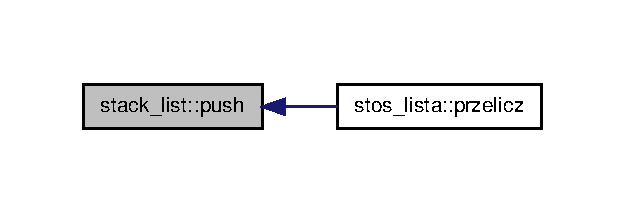
\includegraphics[width=300pt]{classstack__list_a7c8c94a164f180c87fa1d7a8be146a4c_icgraph}
\end{center}
\end{figure}


\hypertarget{classstack__list_adcb1450ccbd547750e6a7939984a7c44}{\index{stack\-\_\-list@{stack\-\_\-list}!size@{size}}
\index{size@{size}!stack_list@{stack\-\_\-list}}
\subsubsection[{size}]{\setlength{\rightskip}{0pt plus 5cm}template$<$typename T\-Y\-P$>$ int {\bf stack\-\_\-list}$<$ T\-Y\-P $>$\-::size (
\begin{DoxyParamCaption}
{}
\end{DoxyParamCaption}
)\hspace{0.3cm}{\ttfamily [inline]}}}\label{classstack__list_adcb1450ccbd547750e6a7939984a7c44}
\begin{DoxyReturn}{Zwraca}
rozmiar ztosu 
\end{DoxyReturn}


Definicja w linii 34 pliku stos.\-hh.



\subsection{Dokumentacja atrybutów składowych}
\hypertarget{classstack__list_a3689c3e1f740bb83ec4471f0487a78a9}{\index{stack\-\_\-list@{stack\-\_\-list}!st@{st}}
\index{st@{st}!stack_list@{stack\-\_\-list}}
\subsubsection[{st}]{\setlength{\rightskip}{0pt plus 5cm}template$<$typename T\-Y\-P$>$ list$<$T\-Y\-P$>$ {\bf stack\-\_\-list}$<$ T\-Y\-P $>$\-::st\hspace{0.3cm}{\ttfamily [private]}}}\label{classstack__list_a3689c3e1f740bb83ec4471f0487a78a9}


Definicja w linii 23 pliku stos.\-hh.



Dokumentacja dla tej klasy została wygenerowana z pliku\-:\begin{DoxyCompactItemize}
\item 
\hyperlink{stos_8hh}{stos.\-hh}\end{DoxyCompactItemize}

\hypertarget{classstos__lista}{\section{\-Dokumentacja klasy stos\-\_\-lista}
\label{classstos__lista}\index{stos\-\_\-lista@{stos\-\_\-lista}}
}


klasa utworzona na potrzeby pomiaru czasu wypełnienia struktury  




{\ttfamily \#include $<$algorytm.\-hh$>$}



\-Diagram dziedziczenia dla stos\-\_\-lista
\nopagebreak
\begin{figure}[H]
\begin{center}
\leavevmode
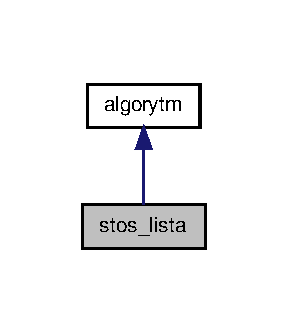
\includegraphics[width=138pt]{classstos__lista__inherit__graph}
\end{center}
\end{figure}


\-Diagram współpracy dla stos\-\_\-lista\-:
\nopagebreak
\begin{figure}[H]
\begin{center}
\leavevmode
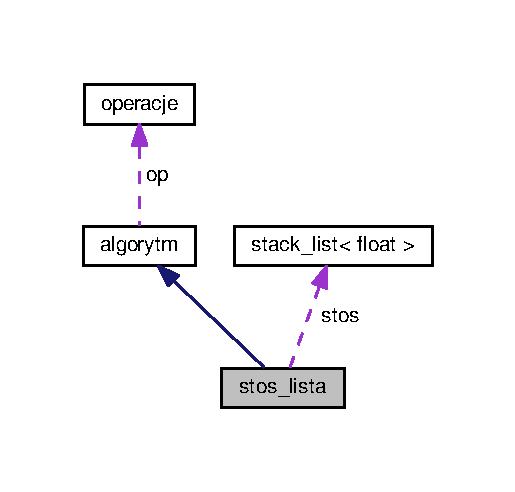
\includegraphics[width=246pt]{classstos__lista__coll__graph}
\end{center}
\end{figure}
\subsection*{\-Metody publiczne}
\begin{DoxyCompactItemize}
\item 
\hyperlink{classstos__lista_ac37fe5bd9067b1283dec0bd241f785f2}{stos\-\_\-lista} (ifstream \&plik1, ifstream \&plik2, int \-N, int \-M)
\item 
float \hyperlink{classstos__lista_a3b0ae65f88cd7760ca7e06f49b57d301}{przelicz} ()
\begin{DoxyCompactList}\small\item\em \-Metoda odpowiada za przetworzenie danych wejsciowych zgodnie z zadanym algorytmem. \end{DoxyCompactList}\end{DoxyCompactItemize}
\subsection*{\-Atrybuty prywatne}
\begin{DoxyCompactItemize}
\item 
\hyperlink{classstack__list}{stack\-\_\-list}$<$ float $>$ \hyperlink{classstos__lista_a94fc88e5b40c7a44e2e34a6f0441853f}{stos}
\end{DoxyCompactItemize}


\subsection{\-Opis szczegółowy}
klasa utworzona na potrzeby pomiaru czasu wypełnienia struktury 

\-Definicja w linii 166 pliku algorytm.\-hh.



\subsection{\-Dokumentacja konstruktora i destruktora}
\hypertarget{classstos__lista_ac37fe5bd9067b1283dec0bd241f785f2}{\index{stos\-\_\-lista@{stos\-\_\-lista}!stos\-\_\-lista@{stos\-\_\-lista}}
\index{stos\-\_\-lista@{stos\-\_\-lista}!stos_lista@{stos\-\_\-lista}}
\subsubsection[{stos\-\_\-lista}]{\setlength{\rightskip}{0pt plus 5cm}{\bf stos\-\_\-lista\-::stos\-\_\-lista} (
\begin{DoxyParamCaption}
\item[{ifstream \&}]{plik1, }
\item[{ifstream \&}]{plik2, }
\item[{int}]{\-N, }
\item[{int}]{\-M}
\end{DoxyParamCaption}
)\hspace{0.3cm}{\ttfamily  \mbox{[}inline\mbox{]}}}}\label{classstos__lista_ac37fe5bd9067b1283dec0bd241f785f2}


\-Definicja w linii 169 pliku algorytm.\-hh.



\subsection{\-Dokumentacja funkcji składowych}
\hypertarget{classstos__lista_a3b0ae65f88cd7760ca7e06f49b57d301}{\index{stos\-\_\-lista@{stos\-\_\-lista}!przelicz@{przelicz}}
\index{przelicz@{przelicz}!stos_lista@{stos\-\_\-lista}}
\subsubsection[{przelicz}]{\setlength{\rightskip}{0pt plus 5cm}float {\bf stos\-\_\-lista\-::przelicz} (
\begin{DoxyParamCaption}
{}
\end{DoxyParamCaption}
)\hspace{0.3cm}{\ttfamily  \mbox{[}virtual\mbox{]}}}}\label{classstos__lista_a3b0ae65f88cd7760ca7e06f49b57d301}


\-Metoda odpowiada za przetworzenie danych wejsciowych zgodnie z zadanym algorytmem. 



\-Reimplementowana z \hyperlink{classalgorytm_af3f92bf537b1f2e1f93173983e838449}{algorytm}.



\-Definicja w linii 135 pliku algorytm.\-cpp.



\-Oto graf wywołań dla tej funkcji\-:
\nopagebreak
\begin{figure}[H]
\begin{center}
\leavevmode
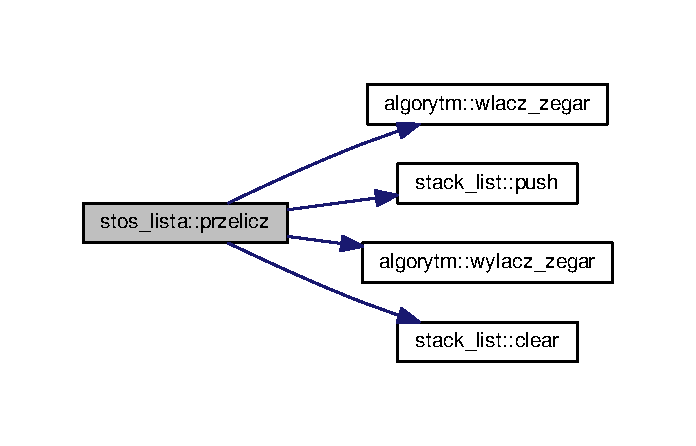
\includegraphics[width=334pt]{classstos__lista_a3b0ae65f88cd7760ca7e06f49b57d301_cgraph}
\end{center}
\end{figure}




\subsection{\-Dokumentacja atrybutów składowych}
\hypertarget{classstos__lista_a94fc88e5b40c7a44e2e34a6f0441853f}{\index{stos\-\_\-lista@{stos\-\_\-lista}!stos@{stos}}
\index{stos@{stos}!stos_lista@{stos\-\_\-lista}}
\subsubsection[{stos}]{\setlength{\rightskip}{0pt plus 5cm}{\bf stack\-\_\-list}$<$float$>$ {\bf stos\-\_\-lista\-::stos}\hspace{0.3cm}{\ttfamily  \mbox{[}private\mbox{]}}}}\label{classstos__lista_a94fc88e5b40c7a44e2e34a6f0441853f}


\-Definicja w linii 167 pliku algorytm.\-hh.



\-Dokumentacja dla tej klasy została wygenerowana z plików\-:\begin{DoxyCompactItemize}
\item 
\hyperlink{algorytm_8hh}{algorytm.\-hh}\item 
\hyperlink{algorytm_8cpp}{algorytm.\-cpp}\end{DoxyCompactItemize}

\hypertarget{classstos__tablica}{\section{\-Dokumentacja klasy stos\-\_\-tablica}
\label{classstos__tablica}\index{stos\-\_\-tablica@{stos\-\_\-tablica}}
}


klasa utworzona na potrzeby pomiaru czasu wypełnienia struktury  




{\ttfamily \#include $<$algorytm.\-hh$>$}



\-Diagram dziedziczenia dla stos\-\_\-tablica\nopagebreak
\begin{figure}[H]
\begin{center}
\leavevmode
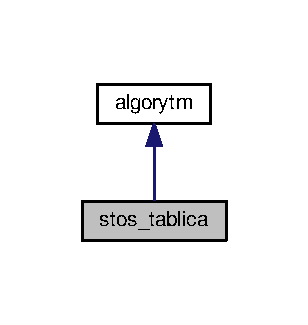
\includegraphics[width=148pt]{classstos__tablica__inherit__graph}
\end{center}
\end{figure}


\-Diagram współpracy dla stos\-\_\-tablica\-:\nopagebreak
\begin{figure}[H]
\begin{center}
\leavevmode
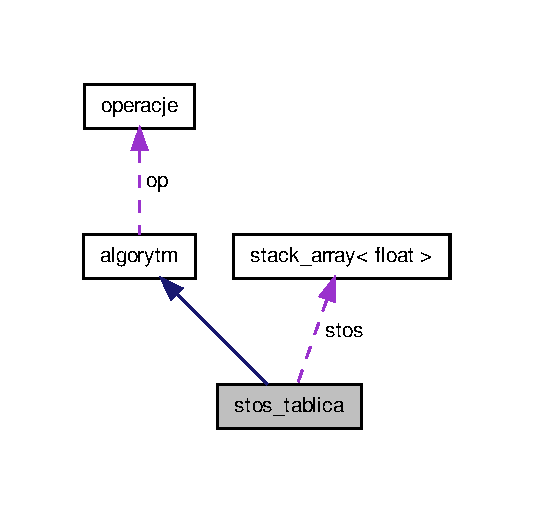
\includegraphics[width=256pt]{classstos__tablica__coll__graph}
\end{center}
\end{figure}
\subsection*{\-Metody publiczne}
\begin{DoxyCompactItemize}
\item 
\hyperlink{classstos__tablica_a74b6909e896922fd4ebb355e1e996523}{stos\-\_\-tablica} (ifstream \&plik1, ifstream \&plik2, int \-N, int \-M, \hyperlink{stos_8hh_a7847560c748814fd3070e9149a9578bd}{flag} \-F)
\begin{DoxyCompactList}\small\item\em konstruktor -\/ ustawia flage w zadany stan \end{DoxyCompactList}\item 
float \hyperlink{classstos__tablica_a44ec89c9723d4034e46ae3b51b01faea}{przelicz} ()
\begin{DoxyCompactList}\small\item\em \-Metoda odpowiada za przetworzenie danych wejsciowych zgodnie z zadanym algorytmem. \end{DoxyCompactList}\end{DoxyCompactItemize}
\subsection*{\-Atrybuty prywatne}
\begin{DoxyCompactItemize}
\item 
\hyperlink{classstack__array}{stack\-\_\-array}$<$ float $>$ \hyperlink{classstos__tablica_a8aa72aa52bd2436cb12d9e1c8e077389}{stos}
\end{DoxyCompactItemize}


\subsection{\-Opis szczegółowy}
klasa utworzona na potrzeby pomiaru czasu wypełnienia struktury 

\-Definicja w linii 153 pliku algorytm.\-hh.



\subsection{\-Dokumentacja konstruktora i destruktora}
\hypertarget{classstos__tablica_a74b6909e896922fd4ebb355e1e996523}{\index{stos\-\_\-tablica@{stos\-\_\-tablica}!stos\-\_\-tablica@{stos\-\_\-tablica}}
\index{stos\-\_\-tablica@{stos\-\_\-tablica}!stos_tablica@{stos\-\_\-tablica}}
\subsubsection[{stos\-\_\-tablica}]{\setlength{\rightskip}{0pt plus 5cm}{\bf stos\-\_\-tablica\-::stos\-\_\-tablica} (
\begin{DoxyParamCaption}
\item[{ifstream \&}]{plik1, }
\item[{ifstream \&}]{plik2, }
\item[{int}]{\-N, }
\item[{int}]{\-M, }
\item[{{\bf flag}}]{\-F}
\end{DoxyParamCaption}
)\hspace{0.3cm}{\ttfamily  \mbox{[}inline\mbox{]}}}}\label{classstos__tablica_a74b6909e896922fd4ebb355e1e996523}


konstruktor -\/ ustawia flage w zadany stan 



\-Definicja w linii 159 pliku algorytm.\-hh.



\subsection{\-Dokumentacja funkcji składowych}
\hypertarget{classstos__tablica_a44ec89c9723d4034e46ae3b51b01faea}{\index{stos\-\_\-tablica@{stos\-\_\-tablica}!przelicz@{przelicz}}
\index{przelicz@{przelicz}!stos_tablica@{stos\-\_\-tablica}}
\subsubsection[{przelicz}]{\setlength{\rightskip}{0pt plus 5cm}float {\bf stos\-\_\-tablica\-::przelicz} (
\begin{DoxyParamCaption}
{}
\end{DoxyParamCaption}
)\hspace{0.3cm}{\ttfamily  \mbox{[}virtual\mbox{]}}}}\label{classstos__tablica_a44ec89c9723d4034e46ae3b51b01faea}


\-Metoda odpowiada za przetworzenie danych wejsciowych zgodnie z zadanym algorytmem. 



\-Reimplementowana z \hyperlink{classalgorytm_af3f92bf537b1f2e1f93173983e838449}{algorytm}.



\-Definicja w linii 106 pliku algorytm.\-cpp.



\-Oto graf wywołań dla tej funkcji\-:\nopagebreak
\begin{figure}[H]
\begin{center}
\leavevmode
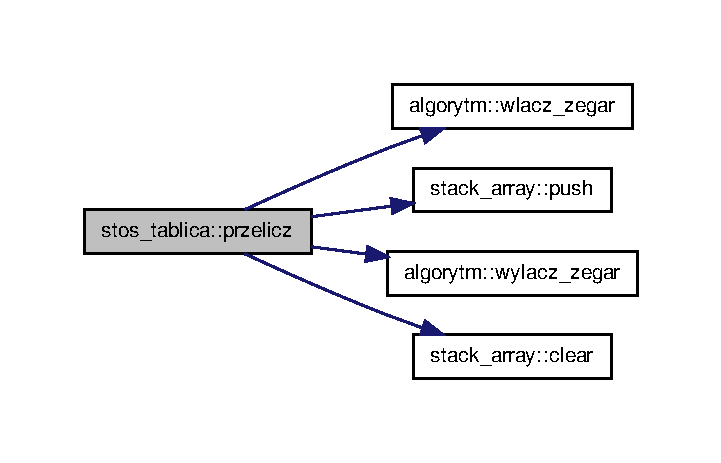
\includegraphics[width=346pt]{classstos__tablica_a44ec89c9723d4034e46ae3b51b01faea_cgraph}
\end{center}
\end{figure}




\subsection{\-Dokumentacja atrybutów składowych}
\hypertarget{classstos__tablica_a8aa72aa52bd2436cb12d9e1c8e077389}{\index{stos\-\_\-tablica@{stos\-\_\-tablica}!stos@{stos}}
\index{stos@{stos}!stos_tablica@{stos\-\_\-tablica}}
\subsubsection[{stos}]{\setlength{\rightskip}{0pt plus 5cm}{\bf stack\-\_\-array}$<$float$>$ {\bf stos\-\_\-tablica\-::stos}\hspace{0.3cm}{\ttfamily  \mbox{[}private\mbox{]}}}}\label{classstos__tablica_a8aa72aa52bd2436cb12d9e1c8e077389}


\-Definicja w linii 154 pliku algorytm.\-hh.



\-Dokumentacja dla tej klasy została wygenerowana z plików\-:\begin{DoxyCompactItemize}
\item 
\hyperlink{algorytm_8hh}{algorytm.\-hh}\item 
\hyperlink{algorytm_8cpp}{algorytm.\-cpp}\end{DoxyCompactItemize}

\chapter{\-Dokumentacja plików}
\hypertarget{algorytm_8cpp}{\section{\-Dokumentacja pliku algorytm.\-cpp}
\label{algorytm_8cpp}\index{algorytm.\-cpp@{algorytm.\-cpp}}
}


plik zawiera definicje metod klas zdefiniowanych w pliku \hyperlink{algorytm_8hh}{algorytm.\-hh}  


{\ttfamily \#include \char`\"{}algorytm.\-hh\char`\"{}}\*
\-Wykres zależności załączania dla algorytm.\-cpp\-:
\nopagebreak
\begin{figure}[H]
\begin{center}
\leavevmode
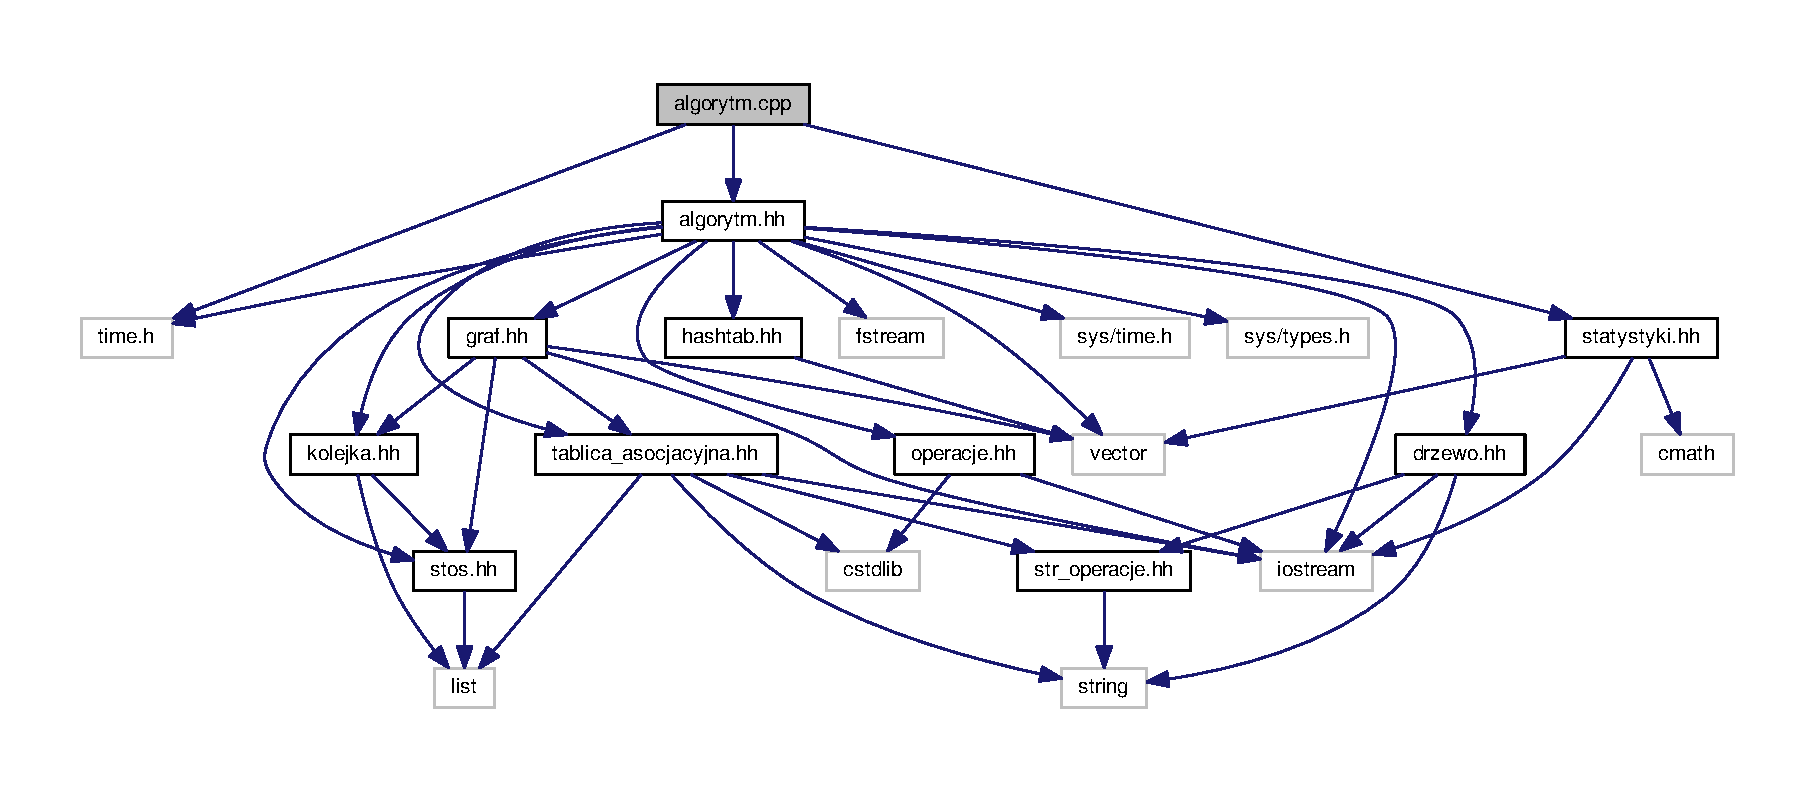
\includegraphics[width=350pt]{algorytm_8cpp__incl}
\end{center}
\end{figure}


\subsection{\-Opis szczegółowy}
plik zawiera definicje metod klas zdefiniowanych w pliku \hyperlink{algorytm_8hh}{algorytm.\-hh} 

\-Definicja w pliku \hyperlink{algorytm_8cpp_source}{algorytm.\-cpp}.


\hypertarget{algorytm_8hh}{\section{\-Dokumentacja pliku algorytm.\-hh}
\label{algorytm_8hh}\index{algorytm.\-hh@{algorytm.\-hh}}
}


\-Definicja klas wykonujacych operacje na zestawie danych wejsciowych.  


{\ttfamily \#include $<$iostream$>$}\*
{\ttfamily \#include $<$fstream$>$}\*
{\ttfamily \#include $<$vector$>$}\*
{\ttfamily \#include $<$ctime$>$}\*
{\ttfamily \#include $<$sys/time.\-h$>$}\*
{\ttfamily \#include $<$sys/types.\-h$>$}\*
\-Wykres zależności załączania dla algorytm.\-hh\-:
\nopagebreak
\begin{figure}[H]
\begin{center}
\leavevmode
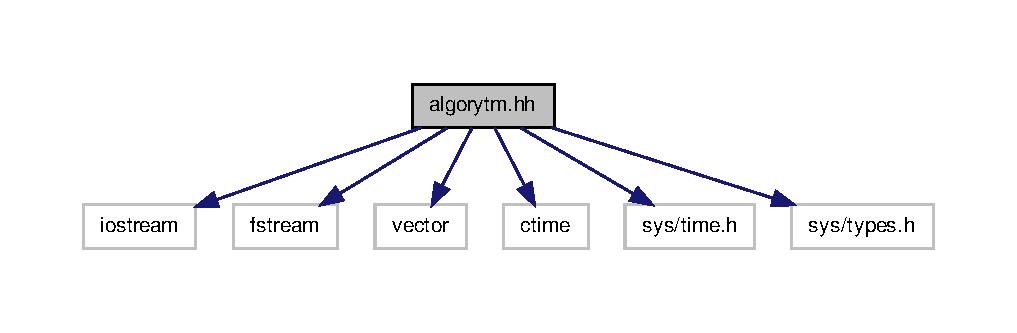
\includegraphics[width=350pt]{algorytm_8hh__incl}
\end{center}
\end{figure}
\-Ten wykres pokazuje, które pliki bezpośrednio lub pośrednio załączają ten plik\-:
\nopagebreak
\begin{figure}[H]
\begin{center}
\leavevmode
\includegraphics[width=226pt]{algorytm_8hh__dep__incl}
\end{center}
\end{figure}
\subsection*{\-Komponenty}
\begin{DoxyCompactItemize}
\item 
class \hyperlink{classalgorytm}{algorytm}
\begin{DoxyCompactList}\small\item\em \-Definicja klasy algorytm \-Jest to klasa bazowa, ktora ma za zadanie wczytac, przetworzyc i porownac plik z plikiem wzorcowym. \end{DoxyCompactList}\item 
class \hyperlink{classmnozenie}{mnozenie}
\begin{DoxyCompactList}\small\item\em modeluje algorytm dokonujacy mnozenia kazdego elementu pliku wejsciowego przez 2 \end{DoxyCompactList}\end{DoxyCompactItemize}


\subsection{\-Opis szczegółowy}
\-Definicja klas wykonujacych operacje na zestawie danych wejsciowych. 

\-Definicja w pliku \hyperlink{algorytm_8hh_source}{algorytm.\-hh}.


\hypertarget{kolejka_8hh}{\section{\-Dokumentacja pliku kolejka.\-hh}
\label{kolejka_8hh}\index{kolejka.\-hh@{kolejka.\-hh}}
}


\-Plik zawiera definicje klasy \-Kolejka \-Zaimplementowanej na 2 sposoby 1. \-Za pomocą listy. 2. \-Za pomocą tablicy a. kazdorazowo powiekszajacej swoj rozmiar b. powiekszajacej swoj rozmiar dwukrotnie, gdy kolejka sie przepelni.  


{\ttfamily \#include $<$list$>$}\*
{\ttfamily \#include \char`\"{}stos.\-hh\char`\"{}}\*
\-Wykres zależności załączania dla kolejka.\-hh\-:
\nopagebreak
\begin{figure}[H]
\begin{center}
\leavevmode
\includegraphics[width=160pt]{kolejka_8hh__incl}
\end{center}
\end{figure}
\-Ten wykres pokazuje, które pliki bezpośrednio lub pośrednio załączają ten plik\-:
\nopagebreak
\begin{figure}[H]
\begin{center}
\leavevmode
\includegraphics[width=226pt]{kolejka_8hh__dep__incl}
\end{center}
\end{figure}
\subsection*{\-Komponenty}
\begin{DoxyCompactItemize}
\item 
class \hyperlink{classqueue__list}{queue\-\_\-list$<$ T\-Y\-P $>$}
\begin{DoxyCompactList}\small\item\em \-Modeluje kolejke oparta na liscie \-S\-T\-L. \end{DoxyCompactList}\item 
class \hyperlink{classqueue__array}{queue\-\_\-array$<$ T\-Y\-P $>$}
\begin{DoxyCompactList}\small\item\em \-Modeluje kolejke w oparciu o tablice. \end{DoxyCompactList}\end{DoxyCompactItemize}


\subsection{\-Opis szczegółowy}
\-Plik zawiera definicje klasy \-Kolejka \-Zaimplementowanej na 2 sposoby 1. \-Za pomocą listy. 2. \-Za pomocą tablicy a. kazdorazowo powiekszajacej swoj rozmiar b. powiekszajacej swoj rozmiar dwukrotnie, gdy kolejka sie przepelni. 

\-Definicja w pliku \hyperlink{kolejka_8hh_source}{kolejka.\-hh}.


\hypertarget{main_8cpp}{\section{Dokumentacja pliku main.\-cpp}
\label{main_8cpp}\index{main.\-cpp@{main.\-cpp}}
}


plik glowny  


{\ttfamily \#include $<$iostream$>$}\\*
{\ttfamily \#include \char`\"{}algorytm.\-hh\char`\"{}}\\*
{\ttfamily \#include \char`\"{}statystyki.\-hh\char`\"{}}\\*
{\ttfamily \#include \char`\"{}operacje.\-hh\char`\"{}}\\*
{\ttfamily \#include \char`\"{}stos.\-hh\char`\"{}}\\*
{\ttfamily \#include \char`\"{}tablica\-\_\-asocjacyjna.\-hh\char`\"{}}\\*
{\ttfamily \#include \char`\"{}drzewo.\-hh\char`\"{}}\\*
{\ttfamily \#include \char`\"{}hashtab.\-hh\char`\"{}}\\*
{\ttfamily \#include \char`\"{}graf.\-hh\char`\"{}}\\*
{\ttfamily \#include $<$cstdlib$>$}\\*
{\ttfamily \#include $<$string$>$}\\*
Wykres zależności załączania dla main.\-cpp\-:\nopagebreak
\begin{figure}[H]
\begin{center}
\leavevmode
\includegraphics[width=350pt]{main_8cpp__incl}
\end{center}
\end{figure}
\subsection*{Funkcje}
\begin{DoxyCompactItemize}
\item 
int \hyperlink{main_8cpp_ae66f6b31b5ad750f1fe042a706a4e3d4}{main} ()
\end{DoxyCompactItemize}


\subsection{Opis szczegółowy}
plik glowny 

Definicja w pliku \hyperlink{main_8cpp_source}{main.\-cpp}.



\subsection{Dokumentacja funkcji}
\hypertarget{main_8cpp_ae66f6b31b5ad750f1fe042a706a4e3d4}{\index{main.\-cpp@{main.\-cpp}!main@{main}}
\index{main@{main}!main.cpp@{main.\-cpp}}
\subsubsection[{main}]{\setlength{\rightskip}{0pt plus 5cm}int main (
\begin{DoxyParamCaption}
{}
\end{DoxyParamCaption}
)}}\label{main_8cpp_ae66f6b31b5ad750f1fe042a706a4e3d4}


Definicja w linii 20 pliku main.\-cpp.



Oto graf wywołań dla tej funkcji\-:\nopagebreak
\begin{figure}[H]
\begin{center}
\leavevmode
\includegraphics[width=350pt]{main_8cpp_ae66f6b31b5ad750f1fe042a706a4e3d4_cgraph}
\end{center}
\end{figure}



\hypertarget{operacje_8cpp}{\section{\-Dokumentacja pliku operacje.\-cpp}
\label{operacje_8cpp}\index{operacje.\-cpp@{operacje.\-cpp}}
}
{\ttfamily \#include \char`\"{}operacje.\-hh\char`\"{}}\*
\-Wykres zależności załączania dla operacje.\-cpp\-:\nopagebreak
\begin{figure}[H]
\begin{center}
\leavevmode
\includegraphics[width=196pt]{operacje_8cpp__incl}
\end{center}
\end{figure}

\hypertarget{operacje_8hh}{\section{\-Dokumentacja pliku operacje.\-hh}
\label{operacje_8hh}\index{operacje.\-hh@{operacje.\-hh}}
}
{\ttfamily \#include $<$cstdlib$>$}\*
{\ttfamily \#include $<$iostream$>$}\*
\-Wykres zależności załączania dla operacje.\-hh\-:
\nopagebreak
\begin{figure}[H]
\begin{center}
\leavevmode
\includegraphics[width=196pt]{operacje_8hh__incl}
\end{center}
\end{figure}
\-Ten wykres pokazuje, które pliki bezpośrednio lub pośrednio załączają ten plik\-:
\nopagebreak
\begin{figure}[H]
\begin{center}
\leavevmode
\includegraphics[width=298pt]{operacje_8hh__dep__incl}
\end{center}
\end{figure}
\subsection*{\-Komponenty}
\begin{DoxyCompactItemize}
\item 
class \hyperlink{classoperacje}{operacje}
\begin{DoxyCompactList}\small\item\em \-Klasa modeluje tablice z danymi i metody sluzace do operacji na niej. \end{DoxyCompactList}\end{DoxyCompactItemize}
\subsection*{\-Definicje}
\begin{DoxyCompactItemize}
\item 
\#define \hyperlink{operacje_8hh_aa50aa866c5823769bb02e986d29a0589}{\-R\-O\-Z\-M\-I\-A\-R}~9
\end{DoxyCompactItemize}


\subsection{\-Dokumentacja definicji}
\hypertarget{operacje_8hh_aa50aa866c5823769bb02e986d29a0589}{\index{operacje.\-hh@{operacje.\-hh}!\-R\-O\-Z\-M\-I\-A\-R@{\-R\-O\-Z\-M\-I\-A\-R}}
\index{\-R\-O\-Z\-M\-I\-A\-R@{\-R\-O\-Z\-M\-I\-A\-R}!operacje.hh@{operacje.\-hh}}
\subsubsection[{\-R\-O\-Z\-M\-I\-A\-R}]{\setlength{\rightskip}{0pt plus 5cm}\#define {\bf \-R\-O\-Z\-M\-I\-A\-R}~9}}\label{operacje_8hh_aa50aa866c5823769bb02e986d29a0589}


\-Definicja w linii 3 pliku operacje.\-hh.


\hypertarget{statystyki_8cpp}{\section{\-Dokumentacja pliku statystyki.\-cpp}
\label{statystyki_8cpp}\index{statystyki.\-cpp@{statystyki.\-cpp}}
}
{\ttfamily \#include \char`\"{}statystyki.\-hh\char`\"{}}\*
\-Wykres zależności załączania dla statystyki.\-cpp\-:\nopagebreak
\begin{figure}[H]
\begin{center}
\leavevmode
\includegraphics[width=258pt]{statystyki_8cpp__incl}
\end{center}
\end{figure}
\subsection*{\-Funkcje}
\begin{DoxyCompactItemize}
\item 
float \hyperlink{statystyki_8cpp_a978b972ebd4a834c47800d668ba8ecf2}{srednia} (float $\ast$tab, int rozmiar)
\begin{DoxyCompactList}\small\item\em funckja oblicza wartosc srednia \end{DoxyCompactList}\item 
float \hyperlink{statystyki_8cpp_a6648f32fbaacb03204231efea979cbf8}{odchylenie\-\_\-standardowe} (float \hyperlink{statystyki_8cpp_a978b972ebd4a834c47800d668ba8ecf2}{srednia}, float $\ast$tab, int rozmiar)
\begin{DoxyCompactList}\small\item\em funckja oblicza odchylenie standardowe \end{DoxyCompactList}\end{DoxyCompactItemize}


\subsection{\-Dokumentacja funkcji}
\hypertarget{statystyki_8cpp_a6648f32fbaacb03204231efea979cbf8}{\index{statystyki.\-cpp@{statystyki.\-cpp}!odchylenie\-\_\-standardowe@{odchylenie\-\_\-standardowe}}
\index{odchylenie\-\_\-standardowe@{odchylenie\-\_\-standardowe}!statystyki.cpp@{statystyki.\-cpp}}
\subsubsection[{odchylenie\-\_\-standardowe}]{\setlength{\rightskip}{0pt plus 5cm}float {\bf odchylenie\-\_\-standardowe} (
\begin{DoxyParamCaption}
\item[{float}]{srednia, }
\item[{float $\ast$}]{tab, }
\item[{int}]{rozmiar}
\end{DoxyParamCaption}
)}}\label{statystyki_8cpp_a6648f32fbaacb03204231efea979cbf8}


funckja oblicza odchylenie standardowe 


\begin{DoxyParams}{\-Parametry}
{\em tab} & -\/ kontener zawierajacy czasy wykonania algorytmu \\
\hline
{\em srednia} & -\/ wartosc srednia \\
\hline
{\em rozmiar} & -\/ rozmiar tablicy \\
\hline
\end{DoxyParams}
\begin{DoxyReturn}{\-Zwraca}
odchylenie standardowe 
\end{DoxyReturn}


\-Definicja w linii 16 pliku statystyki.\-cpp.



\-Oto graf wywoływań tej funkcji\-:\nopagebreak
\begin{figure}[H]
\begin{center}
\leavevmode
\includegraphics[width=350pt]{statystyki_8cpp_a6648f32fbaacb03204231efea979cbf8_icgraph}
\end{center}
\end{figure}


\hypertarget{statystyki_8cpp_a978b972ebd4a834c47800d668ba8ecf2}{\index{statystyki.\-cpp@{statystyki.\-cpp}!srednia@{srednia}}
\index{srednia@{srednia}!statystyki.cpp@{statystyki.\-cpp}}
\subsubsection[{srednia}]{\setlength{\rightskip}{0pt plus 5cm}float {\bf srednia} (
\begin{DoxyParamCaption}
\item[{float $\ast$}]{tab, }
\item[{int}]{rozmiar}
\end{DoxyParamCaption}
)}}\label{statystyki_8cpp_a978b972ebd4a834c47800d668ba8ecf2}


funckja oblicza wartosc srednia 


\begin{DoxyParams}{\-Parametry}
{\em tab} & -\/ kontener zawierajacy czasy wykonania algorytmu \\
\hline
{\em rozmiar} & -\/ rozmiar tablicy \\
\hline
\end{DoxyParams}
\begin{DoxyReturn}{\-Zwraca}
wartosc srednia 
\end{DoxyReturn}


\-Definicja w linii 3 pliku statystyki.\-cpp.



\-Oto graf wywoływań tej funkcji\-:\nopagebreak
\begin{figure}[H]
\begin{center}
\leavevmode
\includegraphics[width=350pt]{statystyki_8cpp_a978b972ebd4a834c47800d668ba8ecf2_icgraph}
\end{center}
\end{figure}



\hypertarget{statystyki_8hh}{\section{\-Dokumentacja pliku statystyki.\-hh}
\label{statystyki_8hh}\index{statystyki.\-hh@{statystyki.\-hh}}
}


plik zawiera dekalracje funkcji odpowiedzialnych za przeprowadznaie statystyk  


{\ttfamily \#include $<$vector$>$}\*
{\ttfamily \#include $<$cmath$>$}\*
{\ttfamily \#include $<$iostream$>$}\*
\-Wykres zależności załączania dla statystyki.\-hh\-:\nopagebreak
\begin{figure}[H]
\begin{center}
\leavevmode
\includegraphics[width=258pt]{statystyki_8hh__incl}
\end{center}
\end{figure}
\-Ten wykres pokazuje, które pliki bezpośrednio lub pośrednio załączają ten plik\-:\nopagebreak
\begin{figure}[H]
\begin{center}
\leavevmode
\includegraphics[width=322pt]{statystyki_8hh__dep__incl}
\end{center}
\end{figure}
\subsection*{\-Funkcje}
\begin{DoxyCompactItemize}
\item 
float \hyperlink{statystyki_8hh_a978b972ebd4a834c47800d668ba8ecf2}{srednia} (float $\ast$tab, int rozmiar)
\begin{DoxyCompactList}\small\item\em funckja oblicza wartosc srednia \end{DoxyCompactList}\item 
float \hyperlink{statystyki_8hh_a6648f32fbaacb03204231efea979cbf8}{odchylenie\-\_\-standardowe} (float \hyperlink{statystyki_8cpp_a978b972ebd4a834c47800d668ba8ecf2}{srednia}, float $\ast$tab, int rozmiar)
\begin{DoxyCompactList}\small\item\em funckja oblicza odchylenie standardowe \end{DoxyCompactList}\end{DoxyCompactItemize}


\subsection{\-Opis szczegółowy}
plik zawiera dekalracje funkcji odpowiedzialnych za przeprowadznaie statystyk 

\-Definicja w pliku \hyperlink{statystyki_8hh_source}{statystyki.\-hh}.



\subsection{\-Dokumentacja funkcji}
\hypertarget{statystyki_8hh_a6648f32fbaacb03204231efea979cbf8}{\index{statystyki.\-hh@{statystyki.\-hh}!odchylenie\-\_\-standardowe@{odchylenie\-\_\-standardowe}}
\index{odchylenie\-\_\-standardowe@{odchylenie\-\_\-standardowe}!statystyki.hh@{statystyki.\-hh}}
\subsubsection[{odchylenie\-\_\-standardowe}]{\setlength{\rightskip}{0pt plus 5cm}float {\bf odchylenie\-\_\-standardowe} (
\begin{DoxyParamCaption}
\item[{float}]{srednia, }
\item[{float $\ast$}]{tab, }
\item[{int}]{rozmiar}
\end{DoxyParamCaption}
)}}\label{statystyki_8hh_a6648f32fbaacb03204231efea979cbf8}


funckja oblicza odchylenie standardowe 


\begin{DoxyParams}{\-Parametry}
{\em tab} & -\/ kontener zawierajacy czasy wykonania algorytmu \\
\hline
{\em srednia} & -\/ wartosc srednia \\
\hline
{\em rozmiar} & -\/ rozmiar tablicy \\
\hline
\end{DoxyParams}
\begin{DoxyReturn}{\-Zwraca}
odchylenie standardowe 
\end{DoxyReturn}


\-Definicja w linii 16 pliku statystyki.\-cpp.



\-Oto graf wywoływań tej funkcji\-:\nopagebreak
\begin{figure}[H]
\begin{center}
\leavevmode
\includegraphics[width=350pt]{statystyki_8hh_a6648f32fbaacb03204231efea979cbf8_icgraph}
\end{center}
\end{figure}


\hypertarget{statystyki_8hh_a978b972ebd4a834c47800d668ba8ecf2}{\index{statystyki.\-hh@{statystyki.\-hh}!srednia@{srednia}}
\index{srednia@{srednia}!statystyki.hh@{statystyki.\-hh}}
\subsubsection[{srednia}]{\setlength{\rightskip}{0pt plus 5cm}float {\bf srednia} (
\begin{DoxyParamCaption}
\item[{float $\ast$}]{tab, }
\item[{int}]{rozmiar}
\end{DoxyParamCaption}
)}}\label{statystyki_8hh_a978b972ebd4a834c47800d668ba8ecf2}


funckja oblicza wartosc srednia 


\begin{DoxyParams}{\-Parametry}
{\em tab} & -\/ kontener zawierajacy czasy wykonania algorytmu \\
\hline
{\em rozmiar} & -\/ rozmiar tablicy \\
\hline
\end{DoxyParams}
\begin{DoxyReturn}{\-Zwraca}
wartosc srednia 
\end{DoxyReturn}


\-Definicja w linii 3 pliku statystyki.\-cpp.



\-Oto graf wywoływań tej funkcji\-:\nopagebreak
\begin{figure}[H]
\begin{center}
\leavevmode
\includegraphics[width=350pt]{statystyki_8hh_a978b972ebd4a834c47800d668ba8ecf2_icgraph}
\end{center}
\end{figure}



\hypertarget{stos_8hh}{\section{\-Dokumentacja pliku stos.\-hh}
\label{stos_8hh}\index{stos.\-hh@{stos.\-hh}}
}


\-Plik zawiera definicje klasy {\ttfamily \-Stos} \-Zaimplementowana na 2 sposoby 1. \-Za pomocą listy. 2. \-Za pomocą tablicy a. kazdorazowo powiekszajacej swoj rozmiar b. powiekszajacej swoj rozmiar dwukrotnie, gdy stos sie przepelni.  


{\ttfamily \#include $<$list$>$}\*
\-Wykres zależności załączania dla stos.\-hh\-:
\nopagebreak
\begin{figure}[H]
\begin{center}
\leavevmode
\includegraphics[width=128pt]{stos_8hh__incl}
\end{center}
\end{figure}
\-Ten wykres pokazuje, które pliki bezpośrednio lub pośrednio załączają ten plik\-:
\nopagebreak
\begin{figure}[H]
\begin{center}
\leavevmode
\includegraphics[width=226pt]{stos_8hh__dep__incl}
\end{center}
\end{figure}
\subsection*{\-Komponenty}
\begin{DoxyCompactItemize}
\item 
class \hyperlink{classstack__list}{stack\-\_\-list$<$ T\-Y\-P $>$}
\begin{DoxyCompactList}\small\item\em \-Modeluje stos oparty na liscie \-S\-T\-L. \end{DoxyCompactList}\item 
class \hyperlink{classstack__array}{stack\-\_\-array$<$ T\-Y\-P $>$}
\begin{DoxyCompactList}\small\item\em \-Modeluje stos w oparciu o tablice. \end{DoxyCompactList}\end{DoxyCompactItemize}
\subsection*{\-Wyliczenia}
\begin{DoxyCompactItemize}
\item 
enum \hyperlink{stos_8hh_a7847560c748814fd3070e9149a9578bd}{flag} \{ \hyperlink{stos_8hh_a7847560c748814fd3070e9149a9578bda4d2a3aa75111d5d02328fb5d495729c2}{plus1}, 
\hyperlink{stos_8hh_a7847560c748814fd3070e9149a9578bdac9b6e8d1af7ce8ae332595ccf954567c}{x2}
 \}
\begin{DoxyCompactList}\small\item\em typ wyliczeniowy sluzacy do ustawienia sposobu zwiekszania pamieci \end{DoxyCompactList}\end{DoxyCompactItemize}


\subsection{\-Opis szczegółowy}
\-Plik zawiera definicje klasy {\ttfamily \-Stos} \-Zaimplementowana na 2 sposoby 1. \-Za pomocą listy. 2. \-Za pomocą tablicy a. kazdorazowo powiekszajacej swoj rozmiar b. powiekszajacej swoj rozmiar dwukrotnie, gdy stos sie przepelni. 

\-Definicja w pliku \hyperlink{stos_8hh_source}{stos.\-hh}.



\subsection{\-Dokumentacja typów wyliczanych}
\hypertarget{stos_8hh_a7847560c748814fd3070e9149a9578bd}{\index{stos.\-hh@{stos.\-hh}!flag@{flag}}
\index{flag@{flag}!stos.hh@{stos.\-hh}}
\subsubsection[{flag}]{\setlength{\rightskip}{0pt plus 5cm}enum {\bf flag}}}\label{stos_8hh_a7847560c748814fd3070e9149a9578bd}


typ wyliczeniowy sluzacy do ustawienia sposobu zwiekszania pamieci 

\begin{Desc}
\item[\-Wartości wyliczeń\-: ]\par
\begin{description}
\index{plus1@{plus1}!stos.\-hh@{stos.\-hh}}\index{stos.\-hh@{stos.\-hh}!plus1@{plus1}}\item[{\em 
\hypertarget{stos_8hh_a7847560c748814fd3070e9149a9578bda4d2a3aa75111d5d02328fb5d495729c2}{plus1}\label{stos_8hh_a7847560c748814fd3070e9149a9578bda4d2a3aa75111d5d02328fb5d495729c2}
}]\index{x2@{x2}!stos.\-hh@{stos.\-hh}}\index{stos.\-hh@{stos.\-hh}!x2@{x2}}\item[{\em 
\hypertarget{stos_8hh_a7847560c748814fd3070e9149a9578bdac9b6e8d1af7ce8ae332595ccf954567c}{x2}\label{stos_8hh_a7847560c748814fd3070e9149a9578bdac9b6e8d1af7ce8ae332595ccf954567c}
}]\end{description}
\end{Desc}



\-Definicja w linii 17 pliku stos.\-hh.


\hypertarget{strona_8dox}{\section{\-Dokumentacja pliku strona.\-dox}
\label{strona_8dox}\index{strona.\-dox@{strona.\-dox}}
}

\printindex
\end{document}
